\def\pgfsysdriver{pgfsys-dvipdfm.def}
\pdfpagewidth=\paperwidth
\pdfpageheight=\paperheight

\documentclass[12pt]{beamer}
\usetheme{Warsaw}

\usepackage{color}
\usepackage{xcolor,colortbl}
\usepackage{indentfirst}
\usepackage[export]{adjustbox}
\usepackage{float}
\usepackage{wrapfig}
\usepackage{setspace}
\usepackage{fontspec}
\usepackage{graphicx}
\usepackage{subcaption}
\usepackage{pgfpages}
\usepackage{amsmath}
\usepackage{bbm}
\usepackage{bm}
\usepackage{dsfont}
\usepackage{xeCJK}
\usepackage[backend=biber]{biblatex}
\usepackage{centernot}

%\setbeamertemplate{footline}{}
\setbeamertemplate{headline}{}
\setbeamertemplate{navigation symbols}{}
%\setbeameroption{show notes on second screen=right}
\setbeamertemplate{note page}[plain]

\addtobeamertemplate{frametitle}{\vspace*{-5pt}}{\vspace*{0pt}}
\setbeamertemplate{section in toc shaded}[default][60]
\setbeamertemplate{subsection in toc shaded}[default][60]

\renewcommand*{\thefootnote}{[\arabic{footnote}]}

\usefonttheme{professionalfonts}

\setsansfont{Open Sans}[Scale=0.75]
\setCJKsansfont[Scale=0.75]{WenQuanYi Micro Hei}

\setbeamerfont{title}{ size={\fontsize{16}{16}} }
%\setbeamerfont{date}{ size={\fontsize{20}{20}} }
\setbeamerfont{note page}{	size={\fontsize{14}{16.8}} }
%\setbeamerfont{note title}{ size = {\fontsize{12}{12}} }
\setbeamerfont{institute}{ size={\fontsize{10}{10}} }
\setbeamerfont{footnote}{ size={\fontsize{9}{9}} }
\setbeamerfont{footline}{ size={\fontsize{7}{7}} }
\setbeamerfont{author}{ size={\fontsize{12}{12}} }
\setbeamerfont{date}{ size={\fontsize{12}{12}} }

\def\dr{\mathrm{d}}

\def\pleq{\preccurlyeq}
\def\pgeq{\succcurlyeq}
\def\pge{\succ}
\def\ple{\prec}

\def\Approx#1{\approx_{#1}}

\def\Span#1{\textbf{Span}\left(#1  \right)}
\def\bvec#1{{\mbox{\boldmath $#1$}}}


\def\prob#1#2{\mbox{Pr}_{#1}\left[ #2 \right]}
\def\pvec#1#2{\vec{\mbox{P}}^{#1}\left[ #2 \right]}
\def\expec#1#2{{\mathbb{E}}_{#1}\left[ #2 \right]}
\def\var#1{\mbox{\bf Var}\left[ #1 \right]}
\newcommand{\E}{\mbox{{\bf E}}}

\def\defeq{\stackrel{\mathrm{def}}{=}}
\def\spliteq{\stackrel{\mathrm{split}}{=}}
\def\setof#1{\left\{#1  \right\}}
\def\sizeof#1{\left|#1  \right|}




\def\floor#1{\left\lfloor #1 \right\rfloor}
\def\ceil#1{\left\lceil #1 \right\rceil}

\def\dim#1{\mathrm{dim} (#1)}
\def\sgn#1{\mathrm{sgn} (#1)}

\def\union{\cup}
\def\intersect{\cap}
\def\Union{\bigcup}
\def\Intersect{\bigcap}

\def\eps{\epsilon}

\def\abs#1{\left|#1  \right|}

\def\trace#1{\mathrm{Tr} \left(#1 \right)}
\def\norm#1{\left\| #1 \right\|}
\def\smallnorm#1{\| #1 \|}


\def\calC{\mathcal{C}}
\def\calE{\mathcal{E}}
\def\calG{\mathcal{G}}
\def\calL{\mathcal{L}}
\def\calS{\mathcal{S}}


\newcommand\Ppsi{\boldsymbol{\mathit{\Psi}}}
\newcommand\ttau{\boldsymbol{\mathit{\tau}}}
\newcommand\PPsi{\boldsymbol{\mathit{\Psi}}}
\newcommand\ppsi{\boldsymbol{\mathit{\psi}}}
\newcommand\pphi{\boldsymbol{\mathit{\phi}}}
\newcommand\Llambda{\boldsymbol{\mathit{\Lambda}}}
\newcommand\PPi{\boldsymbol{\Pi}}

\newcommand\ppi{\boldsymbol{\pi}}
\newcommand\cchi{\boldsymbol{\chi}}
\newcommand\aalpha{\boldsymbol{\alpha}}
\newcommand\bbeta{\boldsymbol{\beta}}
\newcommand\ggamma{\boldsymbol{\gamma}}
\newcommand\ddelta{\boldsymbol{\delta}}

\newcommand\er{R_{\mathrm{eff}}}
\newcommand\ccc{C_{\mathrm{CC}}}
\newcommand\ci{C_{\mathrm{I}}}


\def\aa{\pmb{\mathit{a}}}
\newcommand\bb{\boldsymbol{\mathit{b}}}
\newcommand\cc{\boldsymbol{\mathit{c}}}
\newcommand\dd{\boldsymbol{\mathit{d}}}
\newcommand\ee{\boldsymbol{\mathit{e}}}
\newcommand\ff{\boldsymbol{\mathit{f}}}
\renewcommand\gg{\boldsymbol{\mathit{g}}}
\newcommand\ii{\boldsymbol{\mathit{i}}}
\newcommand\jj{\boldsymbol{\mathit{j}}}
\newcommand\kk{\boldsymbol{\mathit{k}}}
\renewcommand\ll{\boldsymbol{\mathit{l}}}
\newcommand\pp{\boldsymbol{\mathit{p}}}
\newcommand\qq{\boldsymbol{\mathit{q}}}
\newcommand\bs{\boldsymbol{\mathit{s}}}
\newcommand\nn{\boldsymbol{\mathit{n}}}
\newcommand\rr{\boldsymbol{\mathit{r}}}
\renewcommand\ss{\boldsymbol{\mathit{s}}}
\def\tt{\boldsymbol{\mathit{t}}}
\newcommand\uu{\boldsymbol{\mathit{u}}}
\newcommand\vv{\boldsymbol{\mathit{v}}}
\newcommand\ww{\boldsymbol{\mathit{w}}}
\newcommand\yy{\boldsymbol{\mathit{y}}}
\newcommand\zz{\boldsymbol{\mathit{z}}}
\newcommand\xx{\boldsymbol{\mathit{x}}}
\newcommand\xxbar{\overline{\boldsymbol{\mathit{x}}}}

\renewcommand\AA{\boldsymbol{\mathit{A}}}
\newcommand\BB{\boldsymbol{\mathit{B}}}
\newcommand\CC{\boldsymbol{\mathit{C}}}
\newcommand\DD{\boldsymbol{\mathit{D}}}
\newcommand\EE{\boldsymbol{\mathit{E}}}
\newcommand\GG{\boldsymbol{\mathit{G}}}
\newcommand\II{\boldsymbol{\mathit{I}}}
\newcommand\JJ{\boldsymbol{\mathit{J}}}
\newcommand\KK{\boldsymbol{\mathit{K}}}
\newcommand\NN{\boldsymbol{\mathit{N}}}
\newcommand\MM{\boldsymbol{\mathit{M}}}
\newcommand\LL{\boldsymbol{\mathit{L}}}
\newcommand\LH{\boldsymbol{\mathit{H}}}
\newcommand\PP{\boldsymbol{\mathit{P}}}
\newcommand\QQ{\boldsymbol{\mathit{Q}}}
\newcommand\RR{\boldsymbol{\mathit{R}}}
\renewcommand\SS{\boldsymbol{\mathit{S}}}
\newcommand\UU{\boldsymbol{\mathit{U}}}
\newcommand\WW{\boldsymbol{\mathit{W}}}
\newcommand\VV{\boldsymbol{\mathit{V}}}
\newcommand\XX{\boldsymbol{\mathit{X}}}
\newcommand\YY{\boldsymbol{\mathit{Y}}}



\newcommand\MMtil{\boldsymbol{\mathit{\tilde{M}}}}
\newcommand\AAtilde{\boldsymbol{\mathit{\tilde{A}}}}
\newcommand\LLtil{\boldsymbol{\mathit{\tilde{L}}}}
\newcommand\MMtilde{\boldsymbol{\mathit{\tilde{M}}}}

\newcommand\AAn{\boldsymbol{\mathcal{A}}}
\newcommand\ZZ{\boldsymbol{\mathit{Z}}}

\newcommand\AAhat{\boldsymbol{\widehat{\mathit{A}}}}
\newcommand\AAapprox{\boldsymbol{\widetilde{\mathit{A}}}}
\newcommand\DDhat{\boldsymbol{\widehat{\mathit{D}}}}
\newcommand\DDapprox{\boldsymbol{\widetilde{\mathit{D}}}}
\newcommand\LLhat{\boldsymbol{\widehat{\mathit{L}}}}
\newcommand\LLapprox{\boldsymbol{\widetilde{\mathit{L}}}}
\newcommand\MMhat{\boldsymbol{\widehat{\mathit{M}}}}
\newcommand\MMapprox{\boldsymbol{\widetilde{\mathit{M}}}}
\newcommand\ZZhat{\boldsymbol{\widehat{\mathit{Z}}}}

\newcommand\AAtil{\boldsymbol{\widetilde{\mathit{A}}}}
\newcommand\DDtil{\boldsymbol{\widetilde{\mathit{D}}}}


\newcommand\bbtil{\boldsymbol{\tilde{\mathit{b}}}}
\newcommand\xxtil{\boldsymbol{\tilde{\mathit{x}}}}


\newcommand\Otil{\widetilde{O}}

\newcommand\xhat{\boldsymbol{\hat{\mathit{x}}}}
\newcommand\uhat{{\hat{{u}}}}
\newcommand\vhat{{\hat{{v}}}}
\newcommand\what{{\hat{{w}}}}

\newcommand\Ghat{{\widehat{{G}}}}

\newcommand{\sym}[1]{\mathrm{sym} (#1)}

\newcommand{\zero}{\mathbf{0}}
\newcommand{\one}{\mathbf{1}}
\newcommand{\diag}{\textsc{Diag}}
\newcommand\LLs{\boldsymbol{\mathit{L}_s}}

\newcommand{\zztil}{\boldsymbol{\mathit{\widetilde{\zz}}}}
\newcommand{\VVtil}{\boldsymbol{\mathit{\widetilde{V}}}}
\newcommand{\SStil}{\boldsymbol{\mathit{\widetilde{S}}}}
\newcommand{\CCtil}{\boldsymbol{\mathit{\widetilde{C}}}}
\newcommand{\matlowtil}{\boldsymbol{\mathit{\widetilde{\mathcal{L}}}}}
\newcommand{\calDtil}{\boldsymbol{\mathit{\widetilde{\mathcal{D}}}}}
\newcommand{\calCtil}{\boldsymbol{\mathit{\widetilde{\mathcal{C}}}}}
\newcommand{\cctil}{\boldsymbol{\mathit{\widetilde{c}}}}

\newcommand{\SShat}{\boldsymbol{\mathit{\widehat{S}}}}
\newcommand{\CChat}{\boldsymbol{\mathit{\widehat{C}}}}
\newcommand{\matlowhat}{\boldsymbol{\mathit{\widehat{\mathcal{L}}}}}
\newcommand{\calDhat}{\boldsymbol{\mathit{\widehat{\mathcal{D}}}}}
\newcommand{\calChat}{\boldsymbol{\mathit{\widehat{\mathcal{C}}}}}
\newcommand{\cchat}{\boldsymbol{\mathit{\widehat{c}}}}



\newcommand{\calD}{\boldsymbol{\mathit{\mathcal{D}}}}
\renewcommand{\calC}{\boldsymbol{\mathit{\mathcal{C}}}}
%\newcommand\LLtil{\boldsymbol{\mathit{\widetilde{L}}}}

\newcommand{\matlow}{\boldsymbol{\mathit{{\mathcal{L}}}}}

%\newcommand{\PP}{\boldsymbol{\mathit{P}}}

\newcommand{\crunm}{c_1}
\newcommand{\crunn}{c_2}

\newcommand{\todo}[1]{{\bf \color{red} TODO: #1}}
\newcommand{\rp}[1]{{\bf \color{green} RP: #1}}
\newcommand{\hl}[1]{{\bf \color{green} HL: #1}}

\newcommand{\expct}[2]{\ensuremath{\mathop{\text{\normalfont \textbf{E}}}_{#1}}\left[#2\right]}

\DeclareMathOperator*{\argmin}{arg\,min}
\DeclareMathOperator*{\argmax}{arg\,max}

\newcommand{\kh}[1]{\left(#1\right)}

\newcommand{\bsk}{\backslash_\theta}

%\definecolor{Red}{red}{0.95}
\definecolor{Gray}{gray}{0.95}
\definecolor{LightCyan}{rgb}{0.9,1,1}

\newcolumntype{a}{>{\columncolor{LightCyan}}c}
\newcolumntype{b}{>{\columncolor{Gray}}c}


%%%%%%%%%%%%%%%%%%%%%%%%%%%%%%%%%%%%%%%%%%%%%%%%%%%%%%%%%%%%%%%%%%%%%%%%%%%%%%%%%%%%%%%%%%%%%%%%%%%%%%%%%%%%%%%%%%%%%%%%
%%%%%%%%%%%%%%%%%%%%%%%%%%%%%%%%%%%%%%%%%%%%%%%%%%%%%%%%%%%%%%%%%%%%%%%%%%%%%%%%%%%%%%%%%%%%%%%%%%%%%%%%%%%%%%%%%%%%%%%%
%%%%%%%%%%%%%%%%%%%%%%%%%%%%%%%%%%%%%%%%%%%%%%%%%%%%%%%%%%%%%%%%%%%%%%%%%%%%%%%%%%%%%%%%%%%%%%%%%%%%%%%%%%%%%%%%%%%%%%%%
%%%%%%%%%%%%%%%%%%%%%%%%%%%%%%%%%%%%%%%%%%%%%%%%%%%%%%%%%%%%%%%%%%%%%%%%%%%%%%%%%%%%%%%%%%%%%%%%%%%%%%%%%%%%%%%%%%%%%%%%

\title[Kirchhoff Centrality: Nearly Linear Time Algorithms]{Kirchhoff Index As a Measure of Edge Centrality in Weighted Networks: Nearly Linear Time Algorithms}

\author[Huan Li \,\&\, Zhongzhi Zhang]{\quad\\Huan Li\inst{1,2} \and Zhongzhi Zhang\inst{1,2}}

\institute{
	\inst{1}
	School of Computer Science, Fudan University
	\and
	\inst{2}
	Shanghai Key Laboratory of Intelligent Information Processing, Shanghai 200433
	%\inst{4}
	%Laboratoire de Physique Statistique, CNRS UMR 8550, \\
  %Universit\'e P. et M. Curie Paris 6 et \'Ecole Normale Sup\'erieure,
  %24, rue Lhomond, 75005 Paris, France.
	%\and
	%\inst{2}
	%ESPCI and CNRS UMR 7083 Gulliver, 10 rue Vauquelin,Paris 75005
	%\and
	%\inst{3}
	%Institut de Physique Th\'eorique, CEA Saclay and URA 2306, CNRS, 91191 Gif-sur-Yvette, France
}

%\date{ \\[10pt] Speaker:\quad 李\,寰 \vspace{-10pt}}
\date{ \\[10pt] Speaker:\quad Huan\,Li \vspace{-10pt}}

\newcommand{\insfig}[2][1]{
	\begin{figure}
		\includegraphics[width=#1\textwidth]{#2.pdf}
	\end{figure}
}
\newcommand{\cin}{c_{\mathrm{in}}}
\newcommand{\cout}{c_{\mathrm{out}}}
\newcommand{\id}{\mathds{1}}

\graphicspath{{figs/}}

\begin{document}
\begin{spacing}{1.3}

\frame{
	\vspace{15pt}
	\titlepage
}

\frame<0 | handout:0>{
	\frametitle{Outline}
	\begin{itemize}
		\item Kirchhoff index as a centrality measure
			\begin{itemize}
				\item Background of centrality measures and related works
				\item Graph Laplacians, Effective resistances, and Kirchhoff index
				\item Advantages of Kirchhoff index as a centrality measure
			\end{itemize}
		\item Nearly linear time algorithms
			\begin{itemize}
				\item Schur complements, Cholesky factorization, and fast Laplacian solvers
				\item Johnson-Lindenstrauss lemma and Hutchinson's trace estimation
				\item Offline divide and conquer
				\item Sherman-Morrison and Woodbury formulas
			\end{itemize}
	\end{itemize}
}

%\frame{\frametitle{Outline} \tableofcontents}

\section{Kirchhoff Index As a Centrality Measure}

\frame{\frametitle{Outline} \tableofcontents[currentsection]}

\subsection{Background on centrality measures and related works}

\frame{
	\frametitle{Graphs and Networks}
	\begin{itemize}
		\item A graph \small$G = (V,E)$\normalsize\ with 6 vertices and 9 edges 
		{
		\begin{figure}
		\hspace{-20pt}
		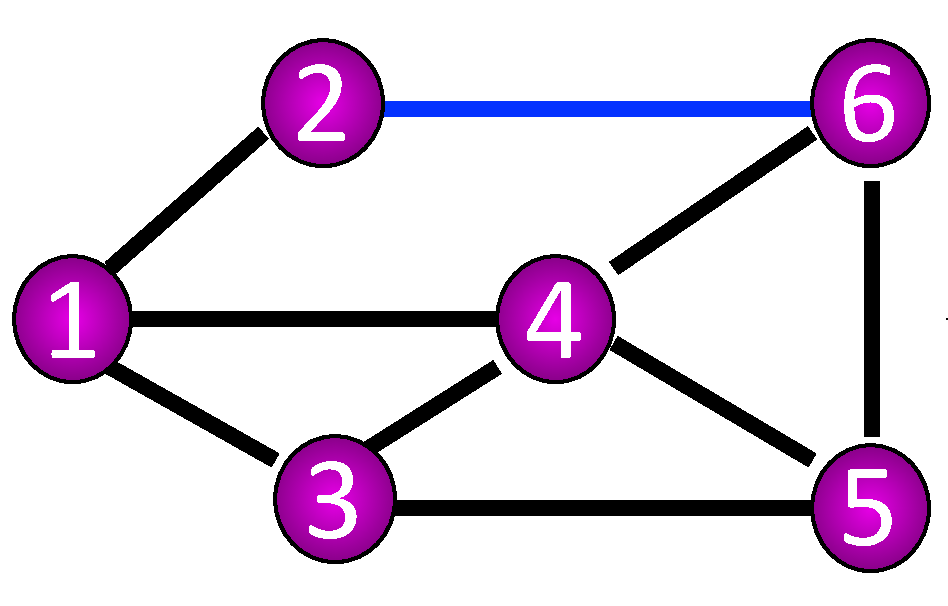
\includegraphics[width=0.45\textwidth]{graph.pdf}
		\end{figure}
		}
	\item Modeling real-world systems by graphs
	\footnotesize
	\begin{table}
		\centering
		%\caption[Caption for LOF]{Some classic real networks.\protect\footnotemark}
		%\caption{Some classic real networks.}
		\begin{tabular}{c|c|c}
			\hline
			\rowcolor{Gray}
			Real-world networks & Vertices & Edges \\
			\hline
			Social networks & People & Friendship/Interactions \\
			\hline
			The World Wide Web & Web pages & Web links \\
			\hline
			Power grid & Stations & Transmission lines \\
			\hline
		\end{tabular}
  \end{table}
  \end{itemize}
  \normalsize
}

\frame{
	\frametitle{Centrality in Networks}
	\vspace{15pt}
	Indicators of \textbf{centrality} identify the most important vertices/edges, e.g.
	\begin{itemize}
		%\item Centrality is often used for detecting
		%	\begin{itemize}
				\item Identify influential persons in a social network
					\begin{itemize}
						\item Independent cascade model%: measuring the importance of a person by its ability in
							%spreading information
					\end{itemize}
				%\item How well used a road is in a transportation network
				\item Identify important web pages in the World Wide Web
					\begin{itemize}
						\item Google's PageRank algorithm%: identifying important web pages by stationary distributions of random walks
					\end{itemize}
				\item Identify important transmission lines in a power grid
		%			\begin{itemize}
		%				\item Northeast blackout of 2003 in Northern America%: failure of a few transmission lines in Cleveland causing
							%a widespread power outage in North America
		%			\end{itemize}
				\begin{figure}
  \begin{minipage}[c]{0.45\textwidth}
    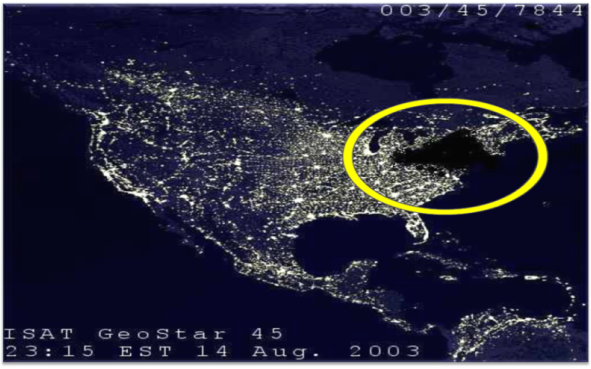
\includegraphics[width=\textwidth]{blackout.png}
  \end{minipage}\hspace{5pt}
  \begin{minipage}[c]{0.4\textwidth}
    \caption{
       Northeast blackout of 2003 in Northern America
    } %\label{fig:03-03}
  \end{minipage}
\end{figure}
		%	\end{itemize}
	\end{itemize}
}

\frame{
	\frametitle{Common Used Edge Centrality Measures}
	\begin{itemize}
		\item Comparing to vertex centrality, edge centrality measures are much less, due to computational challenge
		%\item Common used edge centrality for an edge \small $e \in E$ \normalsize
			\footnotesize
			\begin{table}
				\centering
				%\caption[Caption for LOF]{Some classic real networks.\protect\footnotemark}
				%\caption{Some classic real networks.}
				\begin{tabular}{c|c}
					\hline
					\rowcolor{Gray}
					Edge centrality name & Definition for an edge \scriptsize $e\in E$ \footnotesize \\
					\hline
					Betweenness \scriptsize $\mathcal{B}(e)$ \footnotesize &
						Fraction of shortest paths passing through \scriptsize $e$ \footnotesize \\
					\hline
					Spanning edge centrality \scriptsize $\mathcal{S}(e)$ \footnotesize &
						Fraction of spanning trees containing \scriptsize $e$ \footnotesize \\
					\hline
					Current-flow centrality \scriptsize $\mathcal{F}(e)$ \footnotesize &
						Average current flow passing through \scriptsize $e$ \footnotesize \\
					\hline
				\end{tabular}
		  \end{table}
		  \normalsize
		  
		  \item Weakness
		  	\begin{itemize}
		  		\item Betweenness: only considering shortest paths%, ignoring even slightly longer paths
		  		\item Spanning edge centrality: lacking structure information
		  			\begin{itemize}
		  				\item A path and a star are both trees, while their structures differ
		  			\end{itemize}
				\item Current-flow centrality: hard to compute: \scriptsize$\Otil(mn)$\footnotesize\ running time
		  	\end{itemize}

			%\begin{itemize}
			%	\item Betweenness \[\mathcal{B}(e) \defeq \text{fraction of shortest path passing through} e\]
			%	\item Spanning edge centrality $\mathcal{S}(e) \defeq $
			%\end{itemize}
	\end{itemize}
}

\subsection{Effective resistances and Kirchhoff index}

\frame{
	\frametitle{Effective Resistances (ER)}
	{
	\vspace{-10pt}
	\begin{wrapfigure}{L}{0.4\textwidth}
		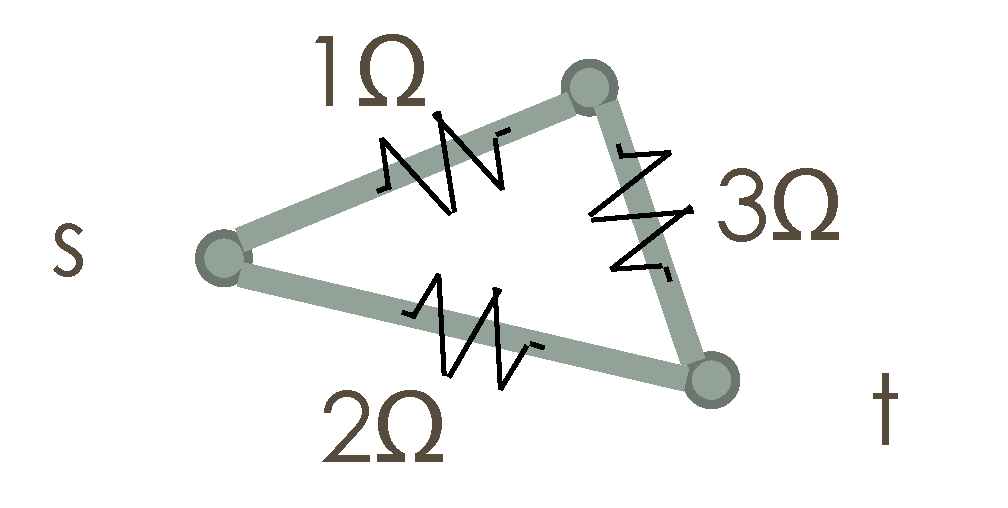
\includegraphics[width=0.4\textwidth]{resistances}
	\end{wrapfigure}
	\quad \\[1pt]
	\small
	\[ \er(s,t) = \frac{1}{\frac{1}{2} + \frac{1}{4}} = \frac{4}{3}\ \Omega \]
	\normalsize
	\quad \\[5pt]
	}
	\quad \\[2.5pt]
	\begin{itemize}
		\item The \textbf{effective resistance} \small$\er(s,t)$ \normalsize between \small$s,t$\, \normalsize is the \textit{electric resistance} between them in the whole electric network%. By Ohm's Law,
			%\small
			%\[
			%	\hspace{-10pt} \er(s,t) = \frac{\vv(s) - \vv(t)}{\ii(s,t)}
			%\]
			%\normalsize
		\item Connection to commute times in random walks
			\begin{itemize}
				\item \small Commute time \footnotesize$\kappa(s,t)$\small : %between
					%\footnotesize$s,t$\,\small\
					expected length of random walk\ % to go from
					\footnotesize$s \to t \to s$\small%, and it is known that
					%\vspace{-12pt}
					\item Relation to ER: \footnotesize
					$
						\kappa(s,t) = \mathrm{vol}(G) \er(s,t)
						%\vspace{-16pt}
					$
					\small
					\vspace{3pt}
					%where \footnotesize$\mathrm{vol}(G)$\small\ is the sum of degrees over all vertices
				\item Thus, \footnotesize$\er(s,t)$\small\ takes into account all paths between \footnotesize$s,t$
			\end{itemize}
	\end{itemize}
}

\frame{
	\frametitle{Kirchhoff Index}
	\begin{itemize}
		\item The \textbf{Kirchhoff index} \small$\mathcal{K}(G)$\normalsize\ %of a graph \small$G$\normalsize\ 
			is defined as% the sum of effective resistances over all vertex pairs, i.e.
			\small
			\vspace{-5pt}
			\[
				\mathcal{K}(G) = \sum\limits_{u,v} \er(u,v)
				\vspace{-5pt}
			\]
			\normalsize
		\item Kirchhoff index takes into account all paths in the graph
		\item Kirchhoff index measures the overall connectivity of the graph
		\item Kirchhoff index has applications to measuring
			\begin{itemize}
				\item The mean cost of search in a complex network
				\item Robustness of first-order consensus algorithm in noisy networks
				\item The global utility of social recommender systems
			\end{itemize}
	\end{itemize}
}

\subsection{Kirchhoff index as a centrality measure and its advantages}

\frame{
	\frametitle{Kirchhoff Centrality}
	\begin{itemize}
		\item Rayleigh's Monotonicity Law
			\begin{itemize}
				\item \footnotesize$\mathcal{K}(G)$\small\ increases when edge conductance is decreased
					%(i.e. edge resistance increased)
				\item Thus, edge (partial) deletion makes the graph less connected
			\end{itemize}
		\item An edge \small$e$\normalsize 's importance is reflected in the increase of Kirchhoff index when $e$ is partially deleted
			\begin{itemize}
				\item Resembling the power grid case
			\end{itemize}
		\item \small$G\bsk e$\,\normalsize\ denotes multiplying conductance of \,\small$e$\,\normalsize\ by
			\small$\theta\in (0, 1/2]$\normalsize
			\footnotesize
			\begin{table}
				\centering
				%\caption[Caption for LOF]{Some classic real networks.\protect\footnotemark}
				%\caption{Some classic real networks.}
				\begin{tabular}{b|c}
					\hline
					\scriptsize$\theta$\footnotesize-Kirchhoff edge centrality \scriptsize$\mathcal{C}_\theta(e)$
					&
						\scriptsize$\mathcal{C}_\theta(e) \defeq \mathcal{K}(G\bsk e)$ \\
					\hline
					\scriptsize$\theta$\footnotesize-Kirchhoff edge centrality \scriptsize$\mathcal{C}_\theta^\Delta(e)$
					&
						\scriptsize$\mathcal{C}_\theta^\Delta(e) \defeq \mathcal{K}(G\bsk e) - \mathcal{K}(G)$ \\
					\hline
					\scriptsize$\theta$\footnotesize-Kirchhoff vertex centrality \scriptsize$\mathcal{C}_\theta^\Delta(v)$
					&
						\scriptsize$\mathcal{C}_\theta^\Delta(v) \defeq \mathcal{K}\kh{G\bsk N(v)} - \mathcal{K}\kh{G}$ \\
					\hline
				\end{tabular}
		  \end{table}
		  \normalsize
	\end{itemize}
}

\frame<0 | handout:0>{
	\frametitle{Comparison With Other Measures}
	\framesubtitle{Examples}
	{
	\vspace{-10pt}
	\begin{wrapfigure}{L}{0.4\textwidth}
		\hspace{10pt}
		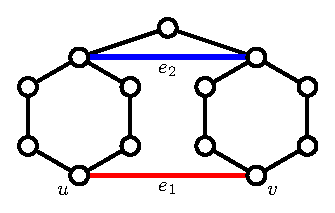
\includegraphics[width=0.4\textwidth]{s_1.eps}
	\end{wrapfigure}
	\quad \\[1pt]
	\small
	\[
		x
	\]
	\normalsize
	\quad \\[5pt]
	}
	\quad \\[20pt]
	{
	%\vspace{-10pt}
	\begin{wrapfigure}{L}{0.6\textwidth}
		\hspace{-20pt}
		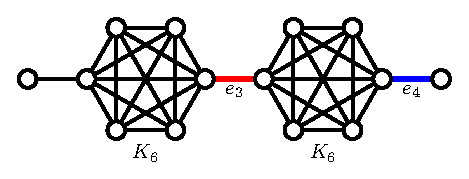
\includegraphics[width=0.6\textwidth]{r_1.eps}
	\end{wrapfigure}
	\quad \\[1pt]
	\small
	\[
		x
	\]
	\normalsize
	\quad \\[5pt]
	}
}

\frame{
	\frametitle{Comparison With Other Measures}
	\framesubtitle{Examples}
	\begin{figure}
		\vspace{10pt}
		\makebox[\linewidth][c]{
		\begin{subfigure}[H]{0.4\textwidth}
			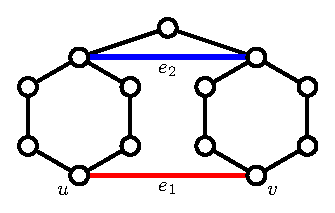
\includegraphics[width=1\textwidth]{s_1.eps}
			%\caption{The first 3 eigenvalues of $B$}
		\end{subfigure}
		\quad\quad\,
		\begin{subfigure}[H]{0.6\textwidth}
			\vspace{10pt}
			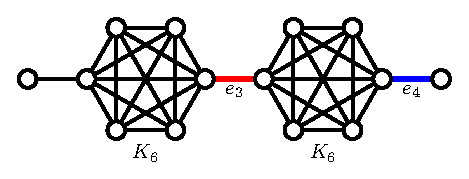
\includegraphics[width=1\textwidth]{r_1.eps}
		\end{subfigure}
		}
		\vspace{2pt}
		%\caption{The accuracy of spectral clustering based on different matrices}
	\end{figure}
	\begin{itemize}
		\item \small Betweenness cannot distinguish between \footnotesize$e_1$\small\ and \footnotesize$e_2$\small
				\footnotesize
				\vspace{-10pt}
				\begin{align*}
					&\mathcal{B}(e_1) = \mathcal{B}(e_2) = 18 \\[0.001cm]
					&\mathcal{C}_{0.1}(e_1) = 132.65,\ \mathcal{C}_{0.1}(e_2) = 112.34
				\end{align*}
				\vspace{-25pt}
		\item \small Spanning edge centrality cannot distinguish between \footnotesize$e_3$\small\ and \footnotesize$e_4$\small
				\footnotesize
				\vspace{-10pt}
				\begin{align*}
					&\mathcal{S}(e_3) = \mathcal{S}(e_4) = 1 \\[0.001cm]
					&\mathcal{C}_{0.1}(e_3) = 467.33,\ \mathcal{C}_{0.1}(e_4) = 197.33
				\end{align*}
				%\vspace{-15pt}
	\end{itemize}
}

\frame{
	\frametitle{Comparison With Other Measures}
	\framesubtitle{Experiments}
	\begin{figure}
		%\vspace{10pt}
		\makebox[\linewidth][c]{
			%\begin{table}
	\centering
	\hspace{-15pt}
	\footnotesize
	\begin{tabular}{|c|c|c|}
		\hline
		\rowcolor{Gray}
		Network name & $\sizeof{V}$ & $\sizeof{E}$ \\
		\hline
		Karate & 34 & 78 \\
		\hline
		Lesmis & 77 & 254 \\
		\hline
		Adjnoun & 112 & 425 \\
		\hline
		Dolphins & 62 & 159 \\
		\hline
		Celegansneural & 297 & 2148 \\
		\hline
	\end{tabular}
	%\end{table}
	\quad
	\begin{subfigure}[H]{0.6\textwidth}
		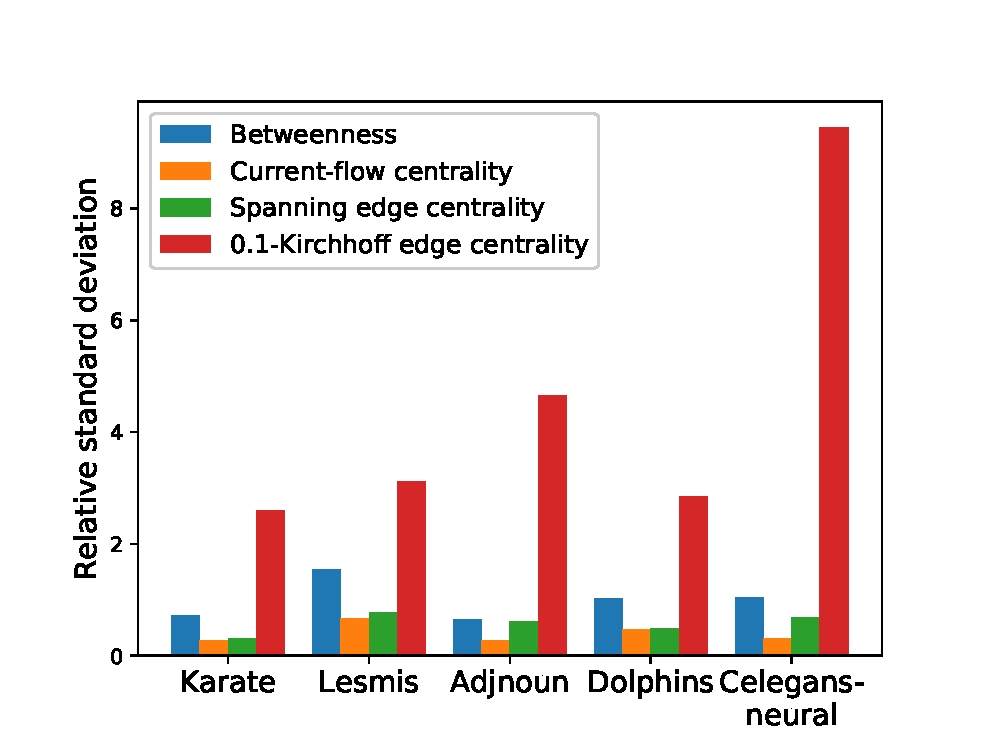
\includegraphics[width=1.2\textwidth]{deviation.eps}
	\end{subfigure}
	}
	\vspace{5pt}
	\end{figure}
%	\small
	\[
		\text{Relative standard deviation} \,\,\defeq \quad \frac{\text{Standard deviation}}{\text{Average}}
	\]
	%}
	%{
	%\begin{wrapfigure}{L}{0.55\textwidth}
%		\hspace{-30pt}
%		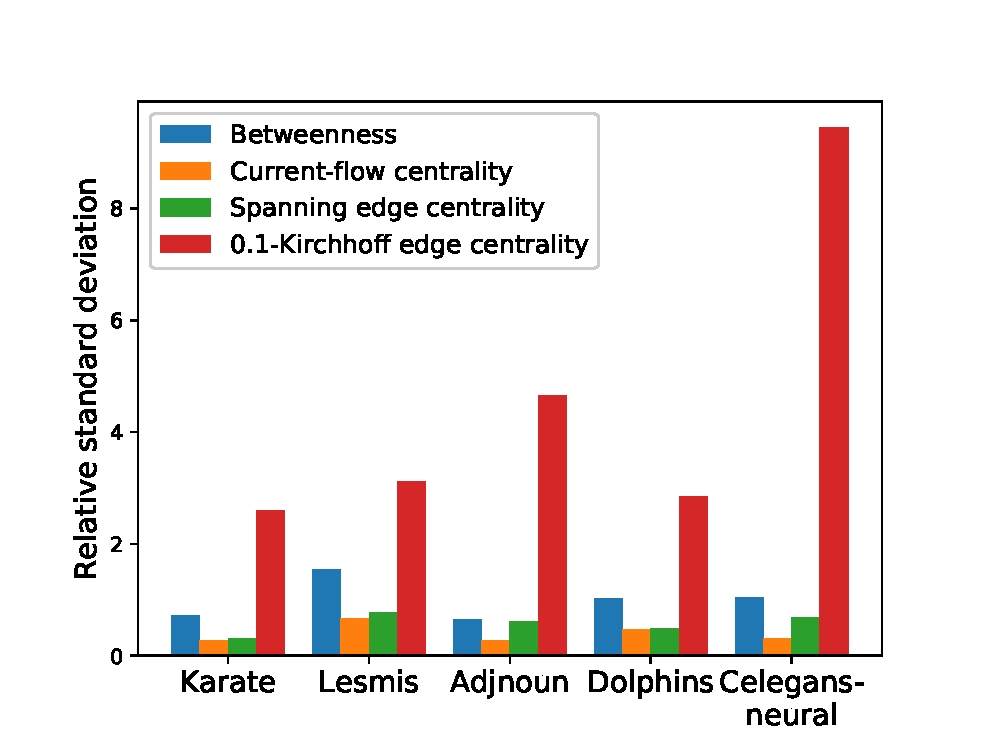
\includegraphics[width=0.7\textwidth]{deviation.eps}
%		\hspace{-30pt}
%	\end{wrapfigure}
%	\quad \\[20pt]
%	\small 
%	\begin{align*}
%		&\text{relative standard deviation}\\
%			\defeq \quad &\frac{\text{standard deviation}}{\text{average}}
%	\end{align*}
%%	\quad \\[5pt]
	%}
}

\section{Nearly Linear Time Algorithms}

\subsection{Approximating\, \footnotesize$%\mathcal{C}_{\theta}(e) \defeq
	\mathcal{K}(G\bsk e)$\,\small\ for
	all \footnotesize$e \in E$\,\small\  in\,\ 
	\footnotesize$\widetilde{O}(m)$\,\small\ time}

\frame{\frametitle{Outline} \tableofcontents[currentsection,currentsubsection]}


			
%\subsection{(Approximate) Schur complements and Cholesky factorization}
%\subsection{Approximate Gaussian elimination for Laplacians}
%\subsection{Johnson-Lindenstrauss lemma and Hutchinson's trace estimation}
%\subsection{Offline divide and conquer}
%\subsection{Sherman-Morrison and Woodbury formulas}

\frame{
	\frametitle{Graph Laplacians}	
	{
	\begin{wrapfigure}{L}{0.58\textwidth}
		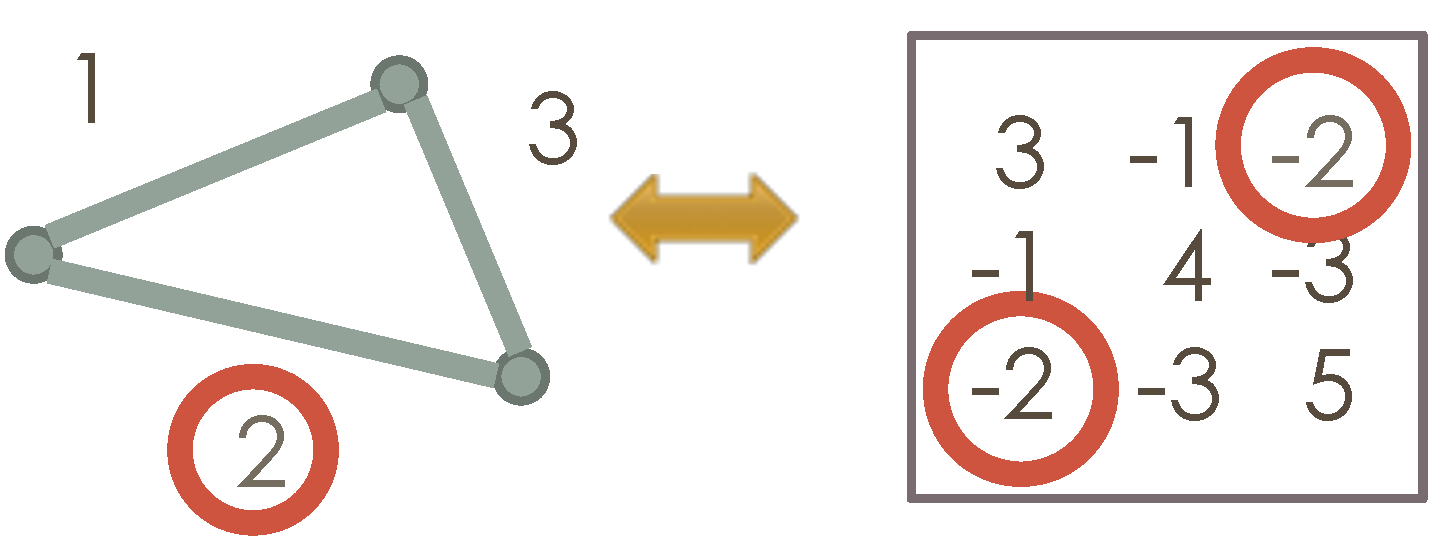
\includegraphics[width=0.5\textwidth]{lapl}
	\end{wrapfigure}
	\quad\\[6pt]
	Coordinates \footnotesize$\Leftrightarrow$\,\ \normalsize Vertices \\
	%\hspace{8.5pt}
	Nonzeros \footnotesize$\Leftrightarrow$\,\ \normalsize Edges
	%\insfig[0.5]{lapl}
	\quad \\[30pt]
	}
	\begin{itemize}
		\item \small Laplacian \footnotesize $\LL_{[u,v]} \ \defeq \ \begin{cases}\sum_{u\neq v} w(u,v) \quad & u = v \\
			- w(u,v) \quad & u \neq v \end{cases}$ \small
		\vspace{6pt}
		\item \footnotesize $\LL$\,\small\ is PSD as \, \footnotesize $\xx^T \LL \xx = \sum\nolimits_{(u,v) \in E} w(u,v)(\xx_u - \xx_v)^2$ \small \vspace{2.5pt}
		\item
		%\footnotesize $\LL = \sum\nolimits_{i=1}^{n} \lambda_i \vv_i \vv_i^T$,\ \,
		Defining pseudoinverse \footnotesize $\LL^\dag$% = \sum\nolimits_{i=2}^{n} \frac{1}{\lambda_i} \vv_i \vv_i^T$
		\small\ \, by inverting all nonzero eigenvalues
%		 where\\[3pt]
%			\begin{itemize}
%				\item \scriptsize$0 = \lambda_1 \leq \lambda_2 \leq\ldots\leq \lambda_n$\,\footnotesize\ 
%					are eigenvalues of \scriptsize$\LL$
%				\item \scriptsize$\one = \vv_1, \vv_2, \ldots, \vv_n$\,\footnotesize\ are the orthonormal eigenvectors
%			\end{itemize}%\vspace{2pt}
		\vspace{4pt}
		\item \footnotesize $\er(u,v) = (\ee_u - \ee_v)^T \LL^\dag (\ee_u - \ee_v)$\,\ ,\quad%\vspace{7pt}
		\footnotesize $\mathcal{K}(G) = n\,\trace{\LL^\dag}$%\vspace{5pt}
	\end{itemize}
}

\frame<0 | handout : 0>{
	\frametitle{Turning Kirchhoff Index into Trace of Pseudoinverse}
	\quad\\[8pt]
	\begin{itemize}
		\item
		\footnotesize $\LL = \sum\nolimits_{i=1}^{n} \lambda_i \vv_i \vv_i^T$,\ \,
		\footnotesize $\LL^\dag = \sum\nolimits_{i=2}^{n} \frac{1}{\lambda_i} \vv_i \vv_i^T$\small\ \, where\\[3pt]
			\begin{itemize}
				\item \scriptsize$0 = \lambda_1 \leq \lambda_2 \leq\ldots\leq \lambda_n$\,\footnotesize\ 
					are eigenvalues of \scriptsize$\LL$
				\item \scriptsize$\one = \vv_1, \vv_2, \ldots, \vv_n$\,\footnotesize\ are the orthonormal eigenvectors
			\end{itemize}\vspace{2pt}
		\item \footnotesize $\er(u,v) = \bb_{u,v}^T \LL^\dag \bb_{u,v}$\vspace{7pt}
		\item \footnotesize $\mathcal{K}(G) = n\,\trace{\LL^\dag}$%\vspace{5pt}
			\scriptsize
			\begin{align*}
				\mathcal{K}(G) &= \sum\limits_{u,v} \er(u,v) = \sum\limits_{u,v} \bb_{u,v}^T \LL^\dag \bb_{u,v} \\
				&= \sum\limits_{u,v} \trace{\LL^\dag \bb_{u,v} \bb_{u,v}^T}
				= \trace{\LL^\dag \sum\limits_{u,v} \bb_{u,v} \bb_{u,v}^T} \\[5pt]
				&= \trace{\LL^\dag \LL_{K_n}} = \trace{\LL^\dag \kh{n\II - \one\one^T}} = n\trace{\LL^\dag}
			\end{align*}
	\end{itemize}
}

\frame{
	\frametitle{Symmetric Gaussian Elimination: Additive View}
	\vspace{20pt}
	\begin{figure}
		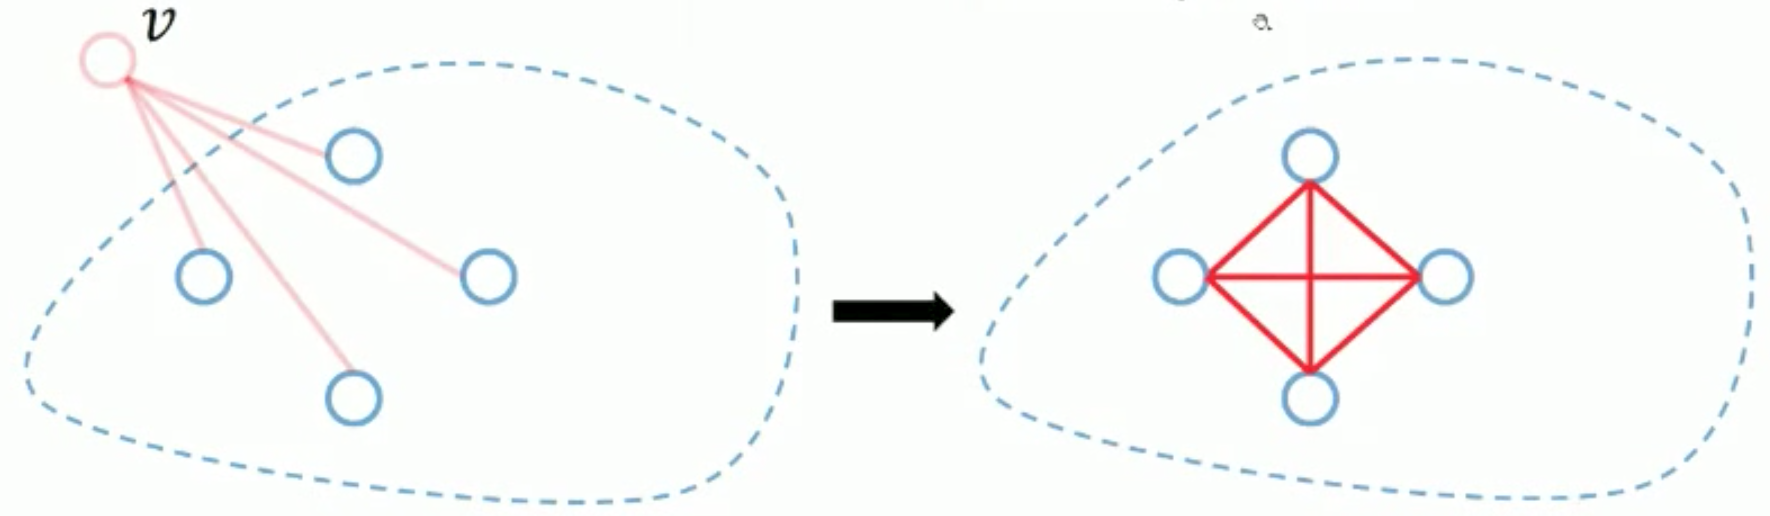
\includegraphics[width=0.7\textwidth]{cliques.png}
	\end{figure}
	%\vspace{-8pt}
	\scriptsize
	\begin{align*}
		\begin{pmatrix}
			4 & -1 & -1 & -1 & -1 \\
			-1 & 1 & 0 & 0 & 0 \\
			-1 & 0 & 1 & 0 & 0 \\
			-1 & 0 & 0 & 1 & 0 \\
			-1 & 0 & 0 & 0 & 1
		\end{pmatrix}
		-
		\frac{1}{4}
		\begin{pmatrix}
		4 \\
		-1 \\
		-1 \\
		-1 \\
		-1
		\end{pmatrix}
		\begin{pmatrix}
		4 \\
		-1 \\
		-1 \\
		-1 \\
		-1
		\end{pmatrix}^T
	%	=\\
	%	\begin{pmatrix}
	%		4 & -1 & -1 & -1 & -1 \\
	%		-1 & 1 & 0 & 0 & 0 \\
	%		-1 & 0 & 1 & 0 & 0 \\
	%		-1 & 0 & 0 & 1 & 0 \\
	%		-1 & 0 & 0 & 0 & 1
	%	\end{pmatrix}
	%	-
	%	\begin{pmatrix}
	%		4 & -1 & -1 & -1 & -1 \\
	%		-1 & \frac{1}{4} & \frac{1}{4} & \frac{1}{4} & \frac{1}{4} \\
	%		-1 & \frac{1}{4} & \frac{1}{4} & \frac{1}{4} & \frac{1}{4} \\
	%		-1 & \frac{1}{4} & \frac{1}{4} & \frac{1}{4} & \frac{1}{4} \\
	%		-1 & \frac{1}{4} & \frac{1}{4} & \frac{1}{4} & \frac{1}{4}
		%\end{pmatrix}
		=
		\begin{pmatrix}
			0 & 0 & 0 & 0 & 0 \\
			0 & \frac{3}{4} & -\frac{1}{4} & -\frac{1}{4} & -\frac{1}{4} \\
			0 & -\frac{1}{4} & \frac{3}{4} & -\frac{1}{4} & -\frac{1}{4} \\
			0 & -\frac{1}{4} & -\frac{1}{4} & \frac{3}{4} & -\frac{1}{4} \\
			0 & -\frac{1}{4} & -\frac{1}{4} & -\frac{1}{4} & \frac{3}{4}
		\end{pmatrix}
	\end{align*}
}

\frame{
	\frametitle{Gaussian Elimination for Laplacians}
	\vspace{7pt}
	\small
	\begin{enumerate}	
		\item Eliminate vertex \,\footnotesize$v_1$\,\small\ (\footnotesize$1^{\text{st}}$\,\small\ row and \,\footnotesize$1^{\text{st}}$\,\small\ column)\,\ by
		\footnotesize \vspace{-7pt}
		\[
			\vspace{-7pt}
			\SS^{(1)} \defeq \LL - \frac{1}{\LL_{[1,1]}} \LL_{[:,1]} \LL_{[:,1]}^T\small
			%\quad \text{\small called the Schur complement w.r.t. \,\footnotesize$v_1$}
		\]
		%where we have \,\footnotesize$\kh{\frac{1}{\LL_{[1,1]}} \LL_{[:,1]} \LL_{[:,1]}^T}_{[1,j]} = \LL_{[1,j]}$\,\small
		\item \footnotesize$\SS^{(1)}$\,\small\ is called the \,\textbf{Schur complement}\,\ w.r.t. \,\footnotesize$v_1$\small
		\vspace{-5pt}
		\item Eliminate vertices \,\footnotesize$v_1,\ldots,v_{n-1}$\,\small\ by
			\footnotesize \vspace{-7pt}
			\[
				\vspace{-12pt}
				\alpha_i = 1 / \SS^{(i-1)}_{[i,i]},\quad\cc_i = \SS^{(i-1)}_{[:,i]},\quad
				\SS^{(i)} = \SS^{(i-1)} - \alpha_i\cc_i\cc_i^T
			\]
			\small
		\item \textbf{Cholesky factorization} \,of \,\footnotesize$\LL=\matlow\calD\matlow^T$\,\small\ 
			\,\footnotesize$\kh{\Rightarrow \LL^\dag=\matlow^{-T}\calD^\dag\matlow^{-1}}$\small
			\footnotesize \vspace{-8pt}
			\[
				\vspace{-8pt}
				\LL = \SS^{(n-1)} + \sum\limits_{i=1}^{n-1} \alpha_i \cc_i\cc_i^T =
				\sum\limits_{i=1}^{n-1} \alpha_i \cc_i\cc_i^T = \matlow\calD\matlow^T
			\]
			\small
			where \,\footnotesize$c_i$\,\small\ is the \,\footnotesize$i^{\text{th}}$\,\small\ column of  \,\footnotesize$\matlow$\,\small,  \,\footnotesize$\alpha_i$\,\small\ is the \,\footnotesize$i^{\text{th}}$\,\small\ diagonal of  \,\footnotesize$\calD$\,\small\ 
	\end{enumerate}
}

%\frame{
%	\frametitle{Gaussian Elimination for Laplacians: An Example}
%}

\frame{
	\frametitle{Approximating Positive Semi-Definite Matrices}
	\begin{itemize}
		%\item \scriptsize$\AA \pleq \BB \quad\Leftrightarrow\quad \forall \xx\in\mathbb{R}^n,\ \xx^T\AA\xx \leq \xx^T\BB\xx$\footnotesize\
		\item \footnotesize Worst-case running time \scriptsize$O(n^3)$:\,\footnotesize\ need to sparsify cliques in Schur complements
		\begin{itemize}
			\item \footnotesize Approximating the clique with a sparser graph
		\end{itemize}
		\item \scriptsize$(1+\eps)$\footnotesize-approximation and \scriptsize$\eps$\footnotesize-approximation
			(\scriptsize$\exp(\eps) \approx 1 + \eps$\footnotesize\ \,for small \scriptsize$\eps$\footnotesize)
		%\vspace{-15pt}
		\begin{table}
			\centering
			%\hspace{-10pt}
			\begin{tabular}{c|c|c}
				\hline
				\rowcolor{Gray}
				Approximation & Nonnegative scalars & PSD Matrices \\
				\hline
				\scriptsize$(1+\eps)$\footnotesize-approx. &
				\scriptsize$(1-\eps)a \leq b \leq (1 + \eps)a$\footnotesize
					&
				\scriptsize$\forall \xx\in\mathbb{R}^n,\ \xx^T \AA \xx \approx_{1 + \eps} \xx^T \BB \xx$\footnotesize\\
				\hline
				\scriptsize$\eps$\footnotesize-approx. &
				\scriptsize$\exp(-\eps) a \leq b \leq \exp(\eps) a$\footnotesize
					&
				\scriptsize$\forall \xx\in\mathbb{R}^n,\ \xx^T \AA \xx \approx_{\eps} \xx^T \BB \xx$\footnotesize\\
				\hline
			\end{tabular}
		\end{table}
		\item \footnotesize For two graphs \scriptsize$G$\,\footnotesize\ and \scriptsize$H$,\,\footnotesize\ 
			\scriptsize$\LL_G \approx_{\eps} \LL_H$\,\footnotesize\ implies
			\begin{enumerate}
				\item \footnotesize All eigenvalues between \scriptsize$\LL_G$\,\footnotesize\ and \scriptsize$\LL_H$\,\footnotesize\ 
					are similar
				\item All cut values between \scriptsize$G$\,\footnotesize\ and \scriptsize$H$\,\footnotesize\ 
					are similar
				\item Random walks in \scriptsize$G$\,\footnotesize\ and \scriptsize$H$\,\footnotesize\ 
					has similar mixing time and cover time
				%\item The solution of linear equations in \scriptsize$\LL_G$\,\footnotesize\ and \scriptsize$\LL_H$\,\footnotesize\ are similar
				\item The inverses are similar, i.e. \scriptsize$\LL_G^\dag \approx_{\eps} \LL_H^\dag$\,\footnotesize\
			\end{enumerate}
%		\item Properties of \scriptsize$\eps$\footnotesize-approximation
%			\begin{enumerate}
%				\item \scriptsize$\AA\approx_\eps \BB, \CC\approx_\eps \DD \quad \Rightarrow \quad 
%					\AA + \CC \approx_\eps \BB + \DD$\footnotesize
%				\item \scriptsize$\AA\approx_\eps \BB \quad \Rightarrow \quad 
%					\VV^T\AA\VV \approx_\eps \VV^T\BB\VV$\footnotesize
%				\item \scriptsize$\AA\approx_{\eps_1} \BB, \BB\approx_{\eps_2} \CC \quad \Rightarrow \quad
%				\AA \approx_{\eps_1 + \eps_2} \CC$\footnotesize
%				\item \scriptsize$\AA\approx_\eps \BB \quad \Rightarrow \quad 
%					\AA^{-1} \approx_\eps \BB^{-1}$\footnotesize
%			\end{enumerate}
%			\vspace{-5pt}
%		\item {\color{red} \scriptsize$\AA\approx_\eps \BB, \CC\approx_\eps \DD \quad \centernot\Rightarrow \quad 
%					\AA - \CC \approx_\eps \BB - \DD$\footnotesize }
%			\vspace{-5pt}
%			\begin{itemize}
%				\item {\color{red} \scriptsize$91\approx_{1.1} 100, 90\approx_{1.1} 90$\footnotesize\ \,
%					but
%					\ \scriptsize$1 \centernot\approx_{1.1} 10$\footnotesize }
%			\end{itemize}
	\end{itemize}
}

\frame{
	\frametitle{Sparsifying Cliques in Schur Complements}
	\vspace{10pt}
	\begin{figure}
		\makebox[\linewidth][c]{
		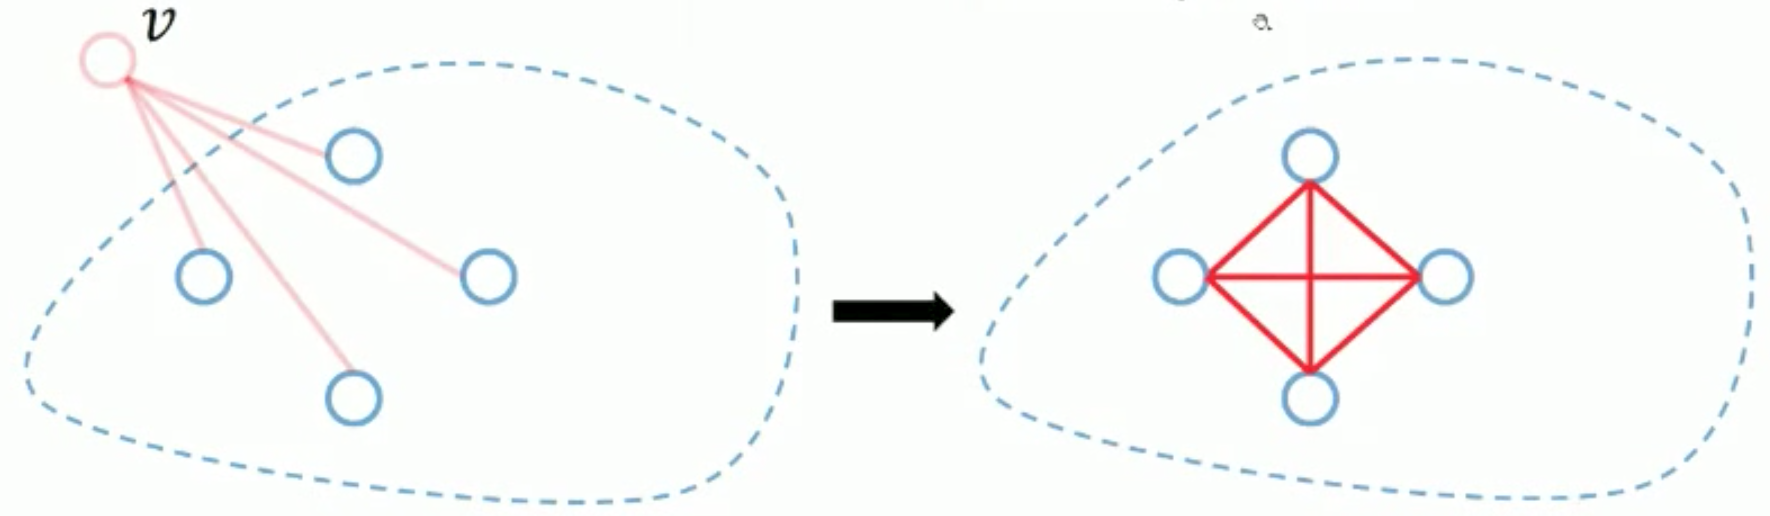
\includegraphics[width=0.7\textwidth]{cliques.png}
		\begin{minipage}[b]{0.07\textwidth}
		\centering
		\small $\approx_\eps$ \normalsize \\[5pt] \quad
		\end{minipage}
		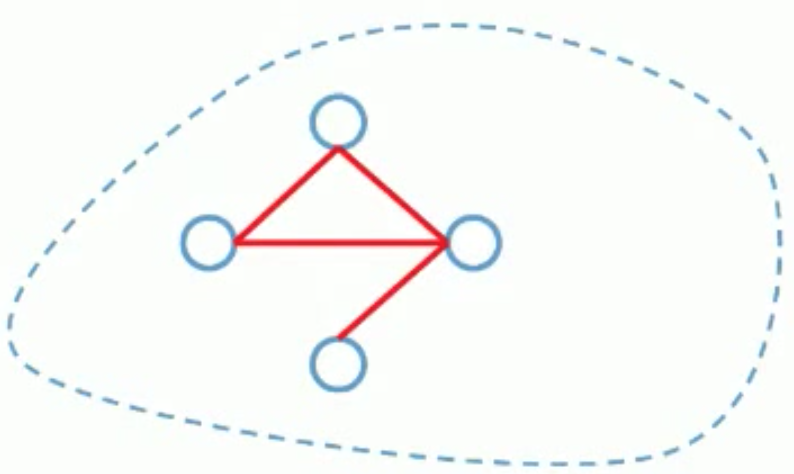
\includegraphics[width=0.3\textwidth]{sparsifier.png}
		}
	\end{figure}
	\vspace{-8pt}
	\small
	\begin{itemize}
		\small
		\item \footnotesize Graph sparsification [SS11]%\footnote[frame]{D. Spielman and S. Srivastava `11.}
			\begin{itemize}
				\vspace{-2.5pt}
				\item \footnotesize Sampling edges by \scriptsize$w(e)\er(e)$\footnotesize\,\ leads to an
					\scriptsize$\widetilde{O}(n)$\footnotesize-edge \scriptsize$\LL_H \approx_\eps \LL_G$\footnotesize\,\ % since
%					\scriptsize\vspace{-8pt}
%					\[
%						\vspace{-8pt}
%						\sum\nolimits_{e\in E} w(e)\er(e) = n - 1
%					\]
%					\footnotesize
			\vspace{-5pt}
			\end{itemize}
		\item \footnotesize Approximate Gaussian elimination [KS16]%\footnote[frame]{R. Kyng and S. Sachdeva `16.}
			\begin{itemize}
				\vspace{-2.5pt}
				\item \footnotesize Sampling edges of the clique by upper bounds of \scriptsize$w(e)\er(e)$\footnotesize\,\ gives a \scriptsize$\deg(v)$\footnotesize-edge sparsifer% \scriptsize$\LH \approx_\eps \LL$\footnotesize
				\item By eliminating vertices in a random order, computes \scriptsize$\LL\approx_\eps \matlow\calD\matlow^T$  
					\footnotesize\ with \scriptsize$\widetilde{O}(m/\eps^2)$\footnotesize\ nonzero entries in \scriptsize$\widetilde{O}(m/\eps^2)$\footnotesize\ time
				\item Enables us to \scriptsize$\eps$\footnotesize -approximate \scriptsize$\zz^T \LL^\dag \zz$\ \footnotesize\ 
					in \scriptsize$\widetilde{O}(m/\eps^2)$\,\footnotesize\ time
			\end{itemize}
	\end{itemize}
}

%\footnote[frame]{\label{KS16}R. Kyng and S. Sachdeva. \textbf{FOCS`16}.}

\frame<0 | handout : 0>
{
	\frametitle{Clique Sampling\footnote[frame]{\label{KS16}R. Kyng and S. Sachdeva. \textbf{FOCS`16}.}}
	\vspace{5pt}
	\begin{itemize}
		\small
		\item Graph sparsification
			\begin{itemize}
				\item \footnotesize Sampling edges by \scriptsize$w(e)\er(e)$\footnotesize\,\ leads to an
					\scriptsize$\widetilde{O}(n)$\footnotesize-edge \scriptsize$\LH \approx_\eps \LL$\footnotesize\,\ since
					\scriptsize\vspace{-8pt}
					\[
						\vspace{-8pt}
						\sum\nolimits_{e\in E} w(e)\er(e) = n - 1
					\]
					\footnotesize
				\item Sampling by \scriptsize$\ttau_e \geq w(e)\er(e)$\footnotesize\,\ leads to an
					\scriptsize$\widetilde{O}(\sum\nolimits_{e\in E}\ttau_e)$\footnotesize-edge \scriptsize$\LH \approx_\eps \LL$\footnotesize
			\end{itemize}
		\item Sparsifying \,\footnotesize$\SS^{(1)} = \LL_{G[V\setminus v_1]} + {\color{red} \sum\limits_{i\sim 1}\sum\limits_{j\sim 1} \frac{w(1,i)w(1,j)}{d}\bb_{i,j}\bb_{i,j}^T}$\small
		\begin{itemize}
			\item \footnotesize  Schur complements preserves ER: \,\scriptsize$\er^{\LL}(i,j) = \er^{\SS^{(1)}}(i,j)$\footnotesize
			\vspace{5pt}
			\item \scriptsize$\er(i,j) \leq \er(1,i) + \er(1,j)\leq \frac{1}{w(1,i)} + \frac{1}{w(1,j)}$\footnotesize
			\vspace{5pt}
			\item Sampling by \scriptsize$\frac{w(1,i)w(1,j)}{d} \kh{\frac{1}{w(1,i)} + \frac{1}{w(1,j)}} =
				\frac{w(1,i) + w(1,j)}{d}$\footnotesize
			\vspace{5pt}
			\item Total edge number \scriptsize$\sum\limits_{i\sim 1}\sum\limits_{j\sim 1} \frac{w(1,i) + w(1,j)}{d}
				= \sizeof{N(v_1)}$
		\end{itemize}
	\end{itemize}
}

\frame<0 | handout : 0>{
	\frametitle{Approximate Gaussian Elimination for Laplacians\footnotemark[1]}
	\small
	\begin{itemize}
		\item Eliminate vertices in random order
			\begin{itemize}
				\item \footnotesize Every step eliminate a vertex with average degree in expectation
				\vspace{5pt}
				\item Total elimination time and total nonzero entries in factorization:
					\scriptsize\vspace{-7pt}
					\[
						\vspace{-7pt}
						\frac{2m}{n} + \frac{2m}{n-1} + \ldots + \frac{2m}{2} = O(m\log n)
					\]\footnotesize
				%\item Number of times an edge is sampled:
				%	\scriptsize\vspace{-8pt}
				%	\[
				%		\vspace{-8pt}
				%		\frac{2}{n} + \frac{2}{n-1} + \ldots + \frac{2}{2} = O(\log n)
				%	\]\footnotesize
				%\vspace{5pt}
				\item Thereby obtain an approximate Cholesky factorization \scriptsize$\LL\approx_\eps \matlow\calD\matlow^T$  
					\footnotesize\ with \scriptsize$\widetilde{O}(m/\eps^2)$\footnotesize\ nonzero entries in \scriptsize$\widetilde{O}(m/\eps^2)$\footnotesize\ time
			\end{itemize}
		\vspace{-5pt}
		\item \footnotesize $\widetilde{O}(m) \defeq O(m\ \mathrm{poly}(\log n))$\small\ \,is called nearly linear time
		\vspace{-5pt}
		\item \small For any vector \footnotesize$\zz \in \mathbb{R}^n$\small, we can compute in \footnotesize$\widetilde{O}(m/\eps^2)$\small\ time
			an \footnotesize$\eps$\small-approximation of \footnotesize$\zz^T\LL^\dag\zz$\small
	\end{itemize}
}

\frame<0 | 0:handout>{
	\frametitle{Solving \large$\LL\xx = \bb$}
}

\frame{
	\frametitle{Estimating Trace of an Implicit Matrix}
%	\begin{block}{Lemma (Hutchinson's Monte-Carlo Trace Estimation)}
%		\scriptsize
%		Let $\AA$ be a $n\times n$ positive semidefinite matrix.
%	Let $\zz_1,\ldots,\zz_M$ be $M$ independent random $\pm 1$ vectors.
%	Let $\eps$ be a scalar such that $0 < \eps \leq 1/2$.
%	For any $M \geq 48\eps^{-2} \ln(2n)$,
%	the following statement holds with probability at least $1 - 1/n$: \vspace{-12pt}
%	\[
%		\frac{1}{M}\sum\limits_{i=1}^M \zz_i^T \AA \zz_i \approx_\eps \trace{\AA}.
%	\]
%	\end{block}
	\vspace{10pt}
	\begin{block}{Hutchinson's Monte-Carlo Trace Estimation
	[Hut89]%\footnote[frame]{Hutchinson `89.}
}
		\vspace{5pt}
		\begin{enumerate}
			\item Let \small $\AA$\,\normalsize\ be a PSD and \small $\zz$\,\normalsize\ be a random \small$\pm 1$\,\normalsize\ vector
			\item \small$\expec{}{\zz^T \AA \zz} = \expec{}{\sum_{u,v}\AA_{[u,v]} \zz_{[u]} \zz_{[v]}} = \trace{\AA}$\,\normalsize\ since\vspace{4pt}
			\begin{itemize}
				\item \scriptsize$\expec{}{\AA_{[u,v]} \zz_{[u]} \zz_{[v]}} = 0$\,\footnotesize\ for \scriptsize$u\neq v$
				\vspace{6pt}
				\item \scriptsize$\expec{}{\AA_{[u,u]} \zz_{[u]}^2} = \AA_{[u,u]}$\,\footnotesize\ for \scriptsize$u = v$
			\end{itemize}
			\item \small$\frac{1}{M}\sum\nolimits_{i=1}^M \zz_i^T \AA \zz_i$\,\normalsize\ 
				should be close to \small$\trace{\AA}$\,\normalsize\ when \small$M$\,\normalsize\ is large
			%\begin{itemize}
				\item \small$O(\log n/\eps^2)$\,\normalsize\ samples are enough to get an	\small$\eps$\normalsize-approximation
				[AT11]
				%\footnote[frame]{Avron and Toledo `11.}
				\begin{itemize}
					\item Derived from Johnson-Lindenstrauss lemma
				\end{itemize}
			%\end{itemize}
		\end{enumerate}
	\end{block}
}

\frame<0 | handout : 0>{
	\frametitle{Estimating Trace by JL}
	\vspace{10pt}
	\begin{block}{Lemma (Johnson-Lindenstrauss)}
		%\begin{lemma}[Johnson-Lindenstrauss]
		\scriptsize
		Given fixed vectors $\vv_1,\vv_2,\cdots,\vv_n \in \mathbb{R}^d$ and $0 < \eps \leq 1/2$, let $k$ be a positive integer such that \vspace{-12pt}
	\[
		\vspace{-12pt}
		%k \geq 24 \eps^{-2} \log n.
		k \geq 4(\eps^2/2 - \eps^3/3)^{-1}\ln n.
	\]
	and $\QQ$ be a $k \times d$ random $\pm 1$ matrix.
	With probability at least $1 - 2 / n$, \vspace{-12pt}
	\[
		%\vspace{-10pt}
		\forall 1\leq i\leq n, \norm{\vv_i}^2_2 \approx_\epsilon \frac{1}{k} \norm{\QQ \vv_i}_2^2.
	\]
	%\end{lemma}
	\end{block}
	\begin{itemize}
		\item \small Proof of number of samples required \vspace{-5pt}
		\scriptsize %\vspace{-5pt}
		\begin{align*}
			\hspace{-5pt}
			\trace{\AA} &= \trace{\AA^{1/2} \AA^{1/2}} = \norm{\AA^{1/2}}_F^2
			\approx_\eps \frac{1}{k}\norm{\QQ_{k\times n}\AA^{1/2}}_F^2 \\
			& = \frac{1}{k}\sum\limits_{i=1}^{k}\norm{\qq_i \AA^{1/2}}_2^2
			= \frac{1}{k}\sum\limits_{i=1}^{k} \kh{\qq_i \AA^{1/2}} \kh{\qq_i \AA^{1/2}}^T
			= \frac{1}{k}\sum\limits_{i=1}^{k} \qq_i\AA \qq_i^T
			%&= \trace{\QQ\AA^{1/2}\AA^{1/2}\QQ^T} = \trace{\QQ\AA\QQ^T}
			%= \sum\limits_{i=1}^{O(\log n / \eps^2)} \qq_i^T\AA \qq_i
		\end{align*}
		\quad\\[-7.5pt]
		\small where \scriptsize$\qq_i$\,\small\ denotes the $i^{\text{th}}$ row of \scriptsize$\QQ$
		%\trace{\AA} &= \trace{\AA^{1/2} \AA^{1/2}} \qquad
			%	\text{\footnotesize since\scriptsize\ $\AA$ \footnotesize is positive semidefinite \scriptsize} \\
			%	&= \sum\limits_{j=1}^{n} \norm{\aa_j}^2_2 \qquad \text{\footnotesize by letting\scriptsize\ $\aa_1,\ldots,\aa_n$\,\footnotesize\ be columns of\scriptsize\ $\AA^{1/2}$} \\
			%	&\approx_{\eps} \sum\limits_{j=1}^{n} \norm{\QQ_{k\times n}\aa_j}^2_2 \qquad
			%		\text{\footnotesize where \scriptsize$k = O(\log n/\eps^2)$} \\
			%	&=
	\end{itemize}
}

\frame{
	\frametitle{Approximating \large$\mathcal{K}(G)$\,\Large\ in Nearly Linear Time}
	\begin{itemize}
		\item Approximating \,\small$\mathcal{K}(G) = n\trace{\LL^\dag}$\normalsize\ \,in \,\footnotesize$\widetilde{O}(m/\eps^4)$\,\normalsize\ time
		\begin{enumerate}
			\item Compute in \footnotesize$\widetilde{O}(m/\eps^2)$\,\small\ time\, \footnotesize$\LL \approx_\eps \matlow \calD \matlow^T$
				with \footnotesize$\widetilde{O}(m/\eps^2)$\,\small\ nonzeros
			\item Generate \footnotesize$M = O(\log n/\eps^2)$\,\small\ independent random \footnotesize$\pm 1$ vectors $\zz_1,\ldots,\zz_M$
			\item Return \footnotesize$\frac{n}{M}\sum\nolimits_{i=1}^M \zz_i^T \matlow^{-T}\calD^\dag \matlow^{-1} \zz_i$\,\small\ as
				an estimate of \footnotesize$\mathcal{K}(G)$
		\end{enumerate}
		\vspace{4pt}
		\item Estimating\, \small$\mathcal{C}_\theta(e) \defeq \mathcal{K}(G\bsk e)$\,\normalsize\ for all \small$e\in E$
			\begin{itemize}
				\item Maintaining \footnotesize$\mathcal{K}(G)$\,\small\ 
					under \footnotesize$O(m)$\,\small\ edge updates
				\item All updates are given beforehand
				\item Processing queries offline: {\color{blue} offline div-conquer}
			\end{itemize}
	\end{itemize}
}

\frame<0 | handout : 0>{
	\frametitle{Offline Div-conquer (离线分治): OI version}
	%\vspace{-5pt}
	\begin{figure}
		\makebox[\linewidth][c]{
		\begin{subfigure}[H]{0.55\textwidth}
			
\includegraphics[width=1\textwidth]{cdq2}
			\label{exp1}	
			\caption{Dynamic programming by div-conquer}
		\end{subfigure}
		\begin{subfigure}[H]{0.55\textwidth}
			\vspace{2.5pt}
			
\includegraphics[width=1\textwidth]{xhr}
			\label{exp2}
			\caption{Div-conquer in query timeline}
		\end{subfigure}
		}
		\\[-2pt]
		\makebox[\linewidth][c]{
		\begin{subfigure}[H]{0.58\textwidth}
			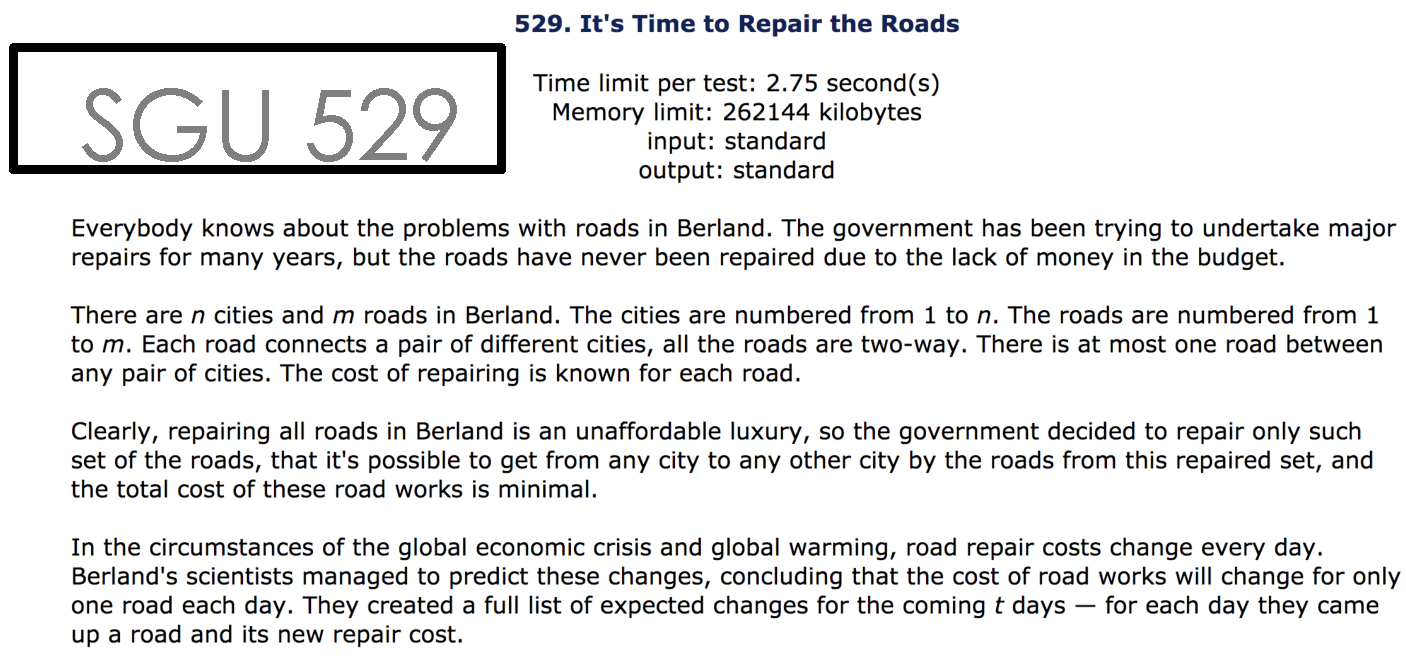
\includegraphics[width=1\textwidth]{sgu_short}
%			\vspace{-25pt}
			\label{exp1}
			\caption{Maintaining MST under updates in \scriptsize$\widetilde{O}(m)$}
		\end{subfigure}
		\begin{subfigure}[H]{0.58\textwidth}
			\vspace{14pt}
			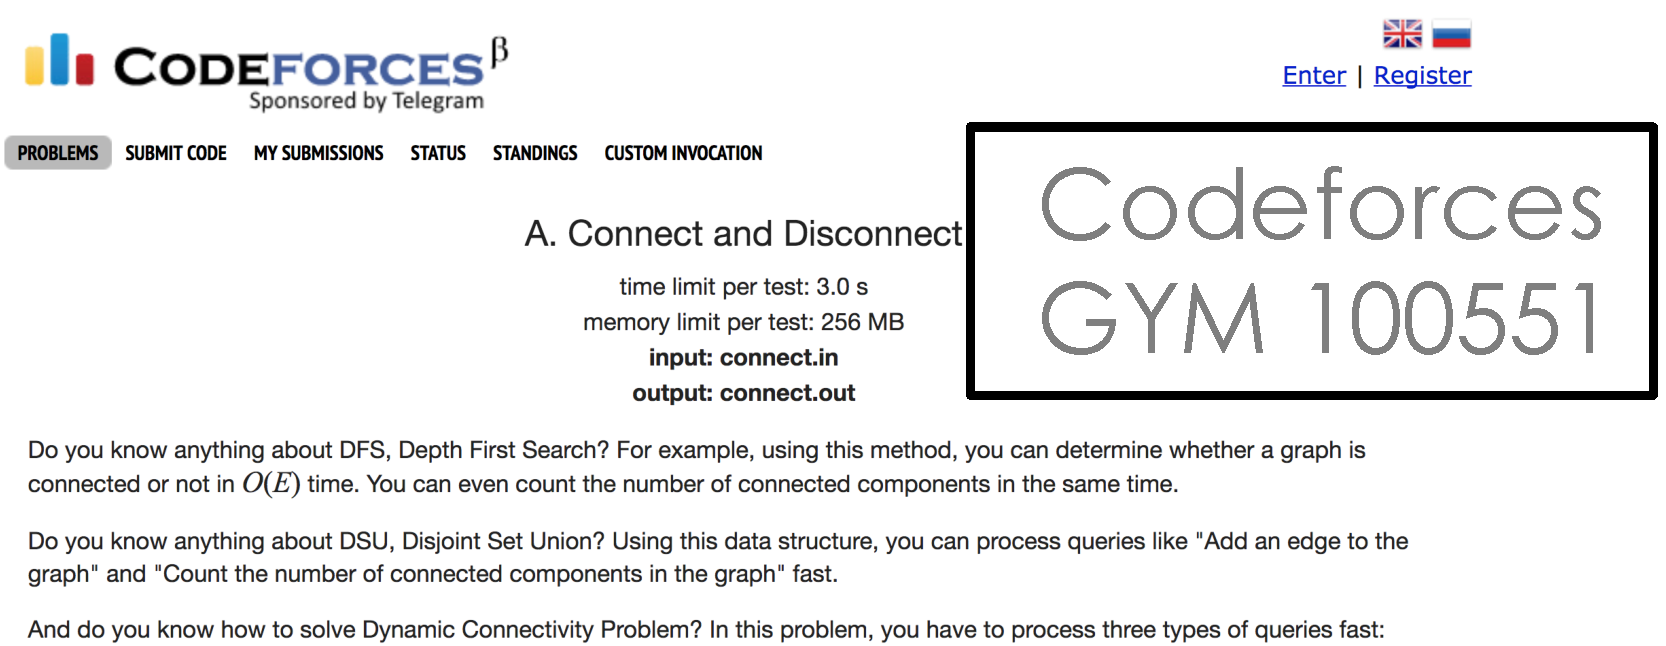
\includegraphics[width=1\textwidth]{cf100551}
			%\vspace{0.1pt}
			\label{exp2}
			\caption{Maintaining \#CC under updates in \scriptsize$\widetilde{O}(m)$}
		\end{subfigure}
		}
		%\caption{The spectrum of $A$ (left) and $B$ (right)}
	\end{figure}
}

\frame<0 | handout : 0>{
	\frametitle{Algorithms That Use Div-conquer}
	\footnotesize
	%\vspace{20pt}
	%\begin{itemize}
		%\item Algorithms that use div-conquer
	\begin{table}\caption{Algorithms that use div-conquer}
		\centering
		%\hspace{-60pt}
		\begin{tabular}{c|c|c}
			\hline
			\rowcolor{Gray}
			Problem & Dense \scriptsize$\kh{m\approx n^2}$\footnotesize & Sparse \scriptsize$\kh{m\approx n}$\footnotesize \\
			\hline
			Determinant &
			\begin{tabular}{c}
					%\hline
					Exact \scriptsize$\widetilde{O}(n^{2.37})$\footnotesize\footnote[frame]{V. V. Williams. \textbf{STOC`12}.} \\
						%\footnote[frame]{D. Durfee, R. Kyng, J. Peebles, A. B. Rao, and S. Sachdeva. \textbf{STOC`17}.} \\
					%\hline
					%\vspace{-5pt}
					Approx. \scriptsize$\widetilde{O}(n^{2})$
					\footnote[frame]{D. Durfee, J. Peebles, R. Peng, and A. B. Rao. \textbf{FOCS`17}.}
				\end{tabular}
			& \scriptsize$\widetilde{O}(n^2)$\footnotesize \footnotesize\footnotemark[3]
				 \\
			\hline
			Rand spanning tree &
				\begin{tabular}{c}
					%\hline
					Exact \scriptsize$\widetilde{O}(n^{5/3}m^{1/3})$\footnotesize
						\footnote[frame]{D. Durfee, R. Kyng, J. Peebles, A. B. Rao, and S. Sachdeva. \textbf{STOC`17}.} \\
					%\hline
					%\vspace{-5pt}
					Approx. \scriptsize$\widetilde{O}(n^{2})$\footnotesize\footnotemark[3]
				\end{tabular}
				&
				\scriptsize$\widetilde{O}(m^{4/3})$\footnotesize
					\footnote[frame]{A. Madry, D. Straszak, and J. Tarnawski. \textbf{SODA`15}.} \\
			\hline
			%Max matching & \scriptsize$O(n^{2.37})$\footnotesize &
			%	\scriptsize$\widetilde{O}(m^{7/4})$\footnotesize \\
			%\hline
			Approx. maxflow & \scriptsize$\widetilde{O}(m)$\footnotesize
				\footnote[frame]{R. Peng. \textbf{SODA`16}.} &
				\scriptsize$\widetilde{O}(m)$\footnotesize\footnotemark[6] \\
			\hline
			\scriptsize$\LL\xx = \bb$\footnotesize & \scriptsize$\widetilde{O}(m)$\footnotesize
				\footnote[frame]{M. B. Cohen, R. Kyng, G. L. Miller, J. W. Pachocki, and R. Peng. \textbf{STOC`14}.} &
				\scriptsize$\widetilde{O}(m)$\footnotesize\footnotemark[7] \\
			\hline
		\end{tabular}
	\end{table}
	%\end{itemize}
}

\frame{
	\frametitle{Partial Cholesky Factorization}
	\vspace{20pt}
	\begin{itemize}
		\item \small Eliminate a set of vertices \,\footnotesize$F = \setof{v_1,\ldots,v_k}$\small\ \,%in random order by
			\footnotesize \vspace{-7pt}
			\[
				\vspace{-7pt}
				\alpha_i = 1 / \SS^{(i-1)}_{[i,i]},\quad\cc_i = \SS^{(i-1)}_{[:,i]},\quad
				\SS^{(i)} = \SS^{(i-1)} - \alpha_i\cc_i\cc_i^T
				\vspace{2.5pt}
			\]
			\small
		\item \textbf{{\color{blue} Partial} Cholesky factorization} (letting \,\footnotesize$C = V - F$\small) %of \,\footnotesize$\LL$\small\ \,
		\footnotesize\vspace{-5pt}
		\[
			\vspace{-5pt}
			\LL = \SS^{(k)} + \sum\limits_{i=1}^k \alpha_i \cc_i \cc_i^T =
			\begin{pmatrix}
				\matlow_{FF} & \zero\\
				\matlow_{CF} & \II_{CC}
			\end{pmatrix}
			\begin{pmatrix}
				\calD & \zero\\
				\zero & \SS
			\end{pmatrix}
			\begin{pmatrix}
				\matlow_{FF} & \zero\\
				\matlow_{CF} & \II_{CC}
			\end{pmatrix}^T
			\vspace{5pt}
		\]\small
		%\vspace{5pt}
		\item \small Recall that elimination of \,\footnotesize$v_1$\,\small\ adds a clique to the remaining graph
%		\small\vspace{-7pt}
%		\[
%			\vspace{-7pt}
%			\SS^{(1)}
%				= \LL_{G[V\setminus v_1]} + \sum\limits_{i\sim 1}\sum\limits_{j\sim 1} \frac{w(1,i)w(1,j)}{d}\bb_{i,j}\bb_{i,j}^T
%		\]
		\vspace{2.5pt}
		\item Commutativity with edge deletions in \,\footnotesize$C$\small\ \,
		\footnotesize\vspace{-7pt}
		\[
			\vspace{-7pt}
			\LL\bsk e =
			\begin{pmatrix}
				\matlow_{FF} & \zero\\
				\matlow_{CF} & \II_{CC}
			\end{pmatrix}
			\begin{pmatrix}
				\calD & \zero\\
				\zero & \SS\bsk e
			\end{pmatrix}
			\begin{pmatrix}
				\matlow_{FF} & \zero\\
				\matlow_{CF} & \II_{CC}
			\end{pmatrix}^T
		\]\small
	\end{itemize}
}

\frame{
	\frametitle{Approximating \large$\zz^T(\LL\bsk e)^\dag\zz$\Large\,\ for all \large$e\in E$\Large\ by Recursion}
	\begin{block}{\small$\textsc{QuadEst}\footnotesize(\LL, \zz, E_Q = E)$: \small Estimate\ \footnotesize$\zz^T(\LL\bsk e)^\dag\zz$\hspace{4pt}\small for all \footnotesize$e\in E_Q$}
		\begin{enumerate}
			\footnotesize
			\item Divide edges in \scriptsize$E_Q$\footnotesize\ into \scriptsize$E^{(1)}, E^{(2)}$\footnotesize\ with equal sizes \vspace{-5pt}
			\item \label{item:start} \footnotesize Let \scriptsize$C$\footnotesize\ denote endpoints of edges in \scriptsize$E^{(1)}$\footnotesize\ and \scriptsize$F = V - C$\footnotesize
			\item Eliminate vertices in \scriptsize$F$\footnotesize\ by clique sampling in random order in nearly linear time:
			\scriptsize\vspace{-8pt}
			\[\vspace{-8pt}
				\LL^\dag \approx_{\eps} 
				\begin{pmatrix}
				\matlow_{FF} & \zero \\
				\matlow_{CF} & \II_{CC}
			\end{pmatrix}^{-T}
			\begin{pmatrix}
				\calD^{-1} & \zero\\
				\zero & {\color{red} \SS^\dag}
			\end{pmatrix}
			\begin{pmatrix}
				\matlow_{FF} & \zero\\
				\matlow_{CF} & \II_{CC}
			\end{pmatrix}^{-1}
			\]
			\footnotesize
			\item Let \scriptsize$\begin{pmatrix}
				\matlow_{FF} & \zero\\
				\matlow_{CF} & \II_{CC}
			\end{pmatrix}^{-1}\zz \defeq \yy \ \spliteq\ \begin{pmatrix} \yy_F \\ \yy_C \end{pmatrix}$\footnotesize,
			then for all \,\scriptsize$e\in E^{(1)}$\footnotesize
			\scriptsize\vspace{-7pt}
			\[
				\vspace{-12pt}
				\zz^T(\LL\bsk e)^\dag\zz = \yy_F^T \calD^{-1}\yy_F + \yy_C^T (\SS\bsk e)^\dag \yy_C
			\]
			\footnotesize
			\item \label{item:end} Sparsify \scriptsize$\SS\,\backslash E^{(1)}$\footnotesize\ and compute
				\scriptsize$\yy_C^T \SS^\dag \yy_C$\footnotesize\ by \,\scriptsize$\footnotesize\textsc{QuadEst}\scriptsize
					(\SS, \yy_C, E^{(1)})$\footnotesize\ \,recursively
			\vspace{-2pt}
			\item Repeat steps~\ref{item:start}\,-\,\ref{item:end} to \scriptsize$E^{(2)}$\footnotesize
			%\vspace{-2pt}
			\item Keep recursing until \scriptsize$\LL$\footnotesize\ only has \scriptsize$O(1)$\footnotesize\ vertices, for which
				calculate \scriptsize
				$
					\zz^T(\LL\bsk e)^\dag\zz
				$
				\footnotesize\ directly for all \scriptsize$e\in E_Q$
		\end{enumerate}
	\end{block}
}

%\frame{
%	\frametitle{Approximating\, \large$\mathcal{C}_{\theta}^\Delta(e) = \mathcal{K}(G\bsk e) - \mathcal{K}(G)$}
%	\begin{itemize}
%%	\end{itemize}
%}

\frame{
	\frametitle{Errors and Running time}	
	\begin{figure}
		\caption{Recursion tree}
		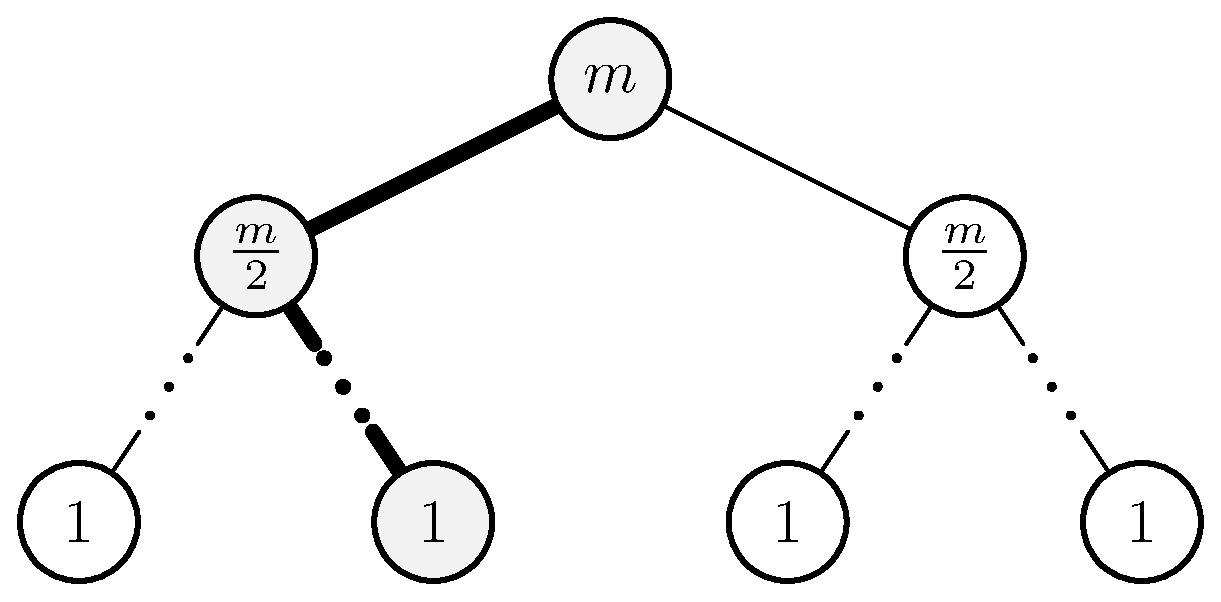
\includegraphics[width = 0.8\textwidth]{l_1.eps}
		\vspace{-5pt}
	\end{figure}
	\begin{itemize}
		\item Set the error of elimination to \small$O(\eps / \log n)$\normalsize\ everywhere
		\item Total running time \small$\widetilde{O}(m/\eps^{4})$
	\end{itemize}
}

\subsection{Approximating\, \footnotesize$%\mathcal{C}_{\theta}^\Delta(e) \defeq
\mathcal{K}(G\bsk e) - \mathcal{K}(G)$\,\small\  for
	all \footnotesize$e \in E$\,\small\  in\,\ 
	\footnotesize$\widetilde{O}(m)$\,\small\ time}
	
\frame{\frametitle{Outline} \tableofcontents[currentsection,currentsubsection]}

\frame{
	\frametitle{Solving \large$\LL\xx = \bb$\,\Large\ in \large$\widetilde{O}(m\log(1/\eps))$\,\Large\ Time}
	\begin{block}{Solving \small$\LL\xx = \bb$\,\normalsize\ by Iterative Refinement}
		\small
		\begin{enumerate}
			\item Computes \footnotesize$\LL \approx_{1/2} \matlow \calD \matlow^T$\,\small\ 
				with \footnotesize$\widetilde{O}(m)$\,\small\ nonzeros in \footnotesize$\widetilde{O}(m)$\,\small\ time
			\item Let \footnotesize$\xx^{(0)} = \zero$\,\small\ and compute\vspace{-5pt}
			\[
				\vspace{-5pt}
				\xx^{(i+1)} \leftarrow \xx^{(i)} - \frac{1}{2}  \matlow^{-T} \calD \matlow^{-1} (\LL \xx^{(i)} - \bb)
			\]
			\item \footnotesize$O(\log(1/\eps))$\,\small\ iterations gives a solution \footnotesize$\hat{x}$\,\small\ satisfying
			\vspace{-5pt}
			\[
				\vspace{-5pt}
				\norm{\hat{\xx} - \xx}_{\LL} \leq \eps \norm{\xx}_{\LL}
			\]
			where \footnotesize$\norm{\xx}_{\LL} = \sqrt{\xx^T \LL \xx}$\small
			\item Total running time \footnotesize$\widetilde{O}(m\log(1/\eps))$
		\end{enumerate}
	\end{block}
}

\frame{
	\frametitle{Equivalent Definitions for Laplacians}
		\begin{figure}
			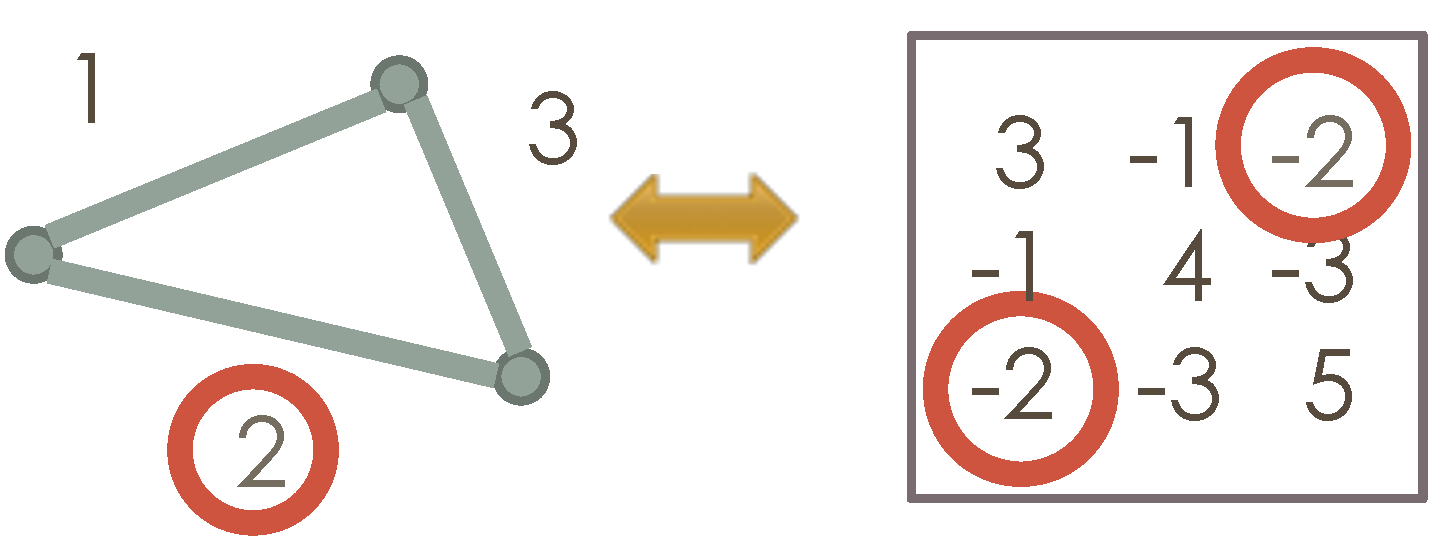
\includegraphics[width=0.5\textwidth]{lapl.pdf}
			\begin{minipage}[b]{0.15\textwidth}
				\centering
				\scriptsize $\quad = \quad \DD - \AA$ \normalsize \\[5pt] \quad
			\end{minipage}
		\end{figure}
		%\insfig[0.5]{lapl}
	\scriptsize
	%\begin{table}
	%	\centering
	%	\begin{tabular}{c|c}
	%		\hline
	\vspace{-12pt}
			\begin{align*}
			\LL 
			&= \sum\limits_{e\in E}w(e) \bb_{e}\bb_{e}^T =
			\begin{pmatrix}
				1 & -1 & 0 \\
				-1 & 1 & 0 \\
				0 & 0 & 0
			\end{pmatrix}
			+
			\begin{pmatrix}
				2 & 0 & -2 \\
				0 & 0 & 0 \\
				-2 & 0 & 2
			\end{pmatrix}
			+
			\begin{pmatrix}
				0 & 0 & 0 \\
				0 & 3 & -3 \\
				0 & -3 & 3
			\end{pmatrix}\\[5pt]
			&= \BB^T \WW \BB =
			\begin{pmatrix}
				1 & 1 & 0 \\
				-1 & 0 & 1 \\
				0 & -1 & -1
			\end{pmatrix}
			\begin{pmatrix}
				1 & 0 & 0 \\
				0 & 2 & 0 \\
				0 & 0 & 3
			\end{pmatrix}
			\begin{pmatrix}
				1 & -1 & 0 \\
				1 & 0 & -1 \\
				0 & 1 & -1
			\end{pmatrix}% \\
			\end{align*}
			%\hline
		%\end{tabular}
	%\end{table}
	\footnotesize
	where\, \scriptsize$\bb_{e} = \bb_{u,v} = \ee_u - \ee_v$\,\footnotesize\ 
	for an edge \scriptsize$e = (u,v) \in E$,\footnotesize\ 
	\scriptsize$\BB^T = \begin{pmatrix} \bb_{1} & \cdots & \bb_{m} \end{pmatrix}$,\footnotesize\ 
	and
	\scriptsize$\WW = \mathrm{Diag}(w(1), \ldots, w(m))$
}

\frame{
	\only<1-1>{\frametitle{Sherman-Morrison}}
	\only<2-2>{\frametitle{Sherman-Morrison (Cont.)}}
	\only<1-1>{\vspace{-2.2pt}}
	\only<2-2>{\vspace{10pt}}
	\begin{itemize}
		\item \footnotesize By Sherman-Morrison formula
		\vspace{-5pt}\scriptsize
		\[
			\vspace{-5pt}
			\kh{\LL - (1 - \theta)\bb_e\bb_e^T}^\dag =
			\LL^\dag + (1 - \theta) \frac{\LL^\dag \bb_e \bb_e^T \LL^\dag}{1 - (1 - \theta)\bb_e^T \LL^\dag \bb_e}
		\]
		\footnotesize
		\only<1-1>{
		\item Approximating the numerator
		\vspace{-5pt}
		\scriptsize
		\[
			\vspace{-5pt}
			\trace{\LL^\dag \bb_e \bb_e^T \LL^\dag} \approx_{\eps}
			\frac{1}{M} \sum\limits_{i=1}^{M} \zz_i^T \LL^\dag \bb_e \bb_e^T \LL^\dag \zz_i
		\]
		\footnotesize
		where \scriptsize$\LL^\dag \zz_i$\,\footnotesize\ can be computed by solving \scriptsize$\LL\xx = \zz_i$\,\footnotesize\ 
		\vspace{5pt}
		\item {\color{blue} Lemma:} \scriptsize$\norm{\hat{\yy}_i - \LL^\dag \zz_i}_{\LL} \leq \frac{1}{36}\eps / n^{7}$\,\footnotesize\ gives
		\scriptsize
		\vspace{-5pt}
		\[
			\vspace{-5pt}
			\sum\limits_{i=1}^{M} \hat{\yy}_i^T \bb_e \bb_e^T \hat{\yy}_i
			\approx_{\eps}
			\trace{\LL^\dag \bb_e \bb_e^T \LL^\dag}
		\]
		\footnotesize
		(Derived from polynomial bounds on eigenvalues of \scriptsize$\LL$\footnotesize)
		}
		\only<2-2>{
			\item Approximating the denominator \scriptsize$1 - (1-\theta)\er(e)$\footnotesize
			\begin{itemize}
				\item \scriptsize$\hat{r}_e \approx_\eps \er(e) \quad\Rightarrow\quad
					1 - (1-\theta)\hat{r}_e \approx_{3\eps/\theta} 1 - (1-\theta)\er(e)$\footnotesize
				\item \scriptsize$\abs{\hat{r}_e - \er(e)} \leq 2\eps \er(e)$\footnotesize
				\vspace{2.5pt}
				\item \scriptsize$\er(e) \leq 1 \quad \Rightarrow 1 - (1 - \theta)\er(e) \geq \theta \er(e)$
			\end{itemize}
			\vspace{5pt}
			\item Approximating \scriptsize$\er(e)$\,\footnotesize\ for all \scriptsize$e \in E$\,\footnotesize\ in
				\scriptsize$\widetilde{O}(m/\eps^2)$\,\footnotesize\ time [SS11]
				\vspace{-5pt}
				\scriptsize
				\begin{align*}
					\er(e) &= \bb_e^T \LL^\dag \bb_e = \bb_e^T \LL^\dag \LL \LL^\dag \bb_e = \bb_e \LL^\dag \BB^T \BB \LL^\dag \bb_e
					\\ &= \trace{\BB\LL^\dag \bb_e \bb_e^T \LL^\dag \BB^T}
					\approx_{\eps} \sum\limits_{i=1}^{M} \zz_i^T \BB\LL^\dag \bb_e \bb_e^T \LL^\dag \BB^T \zz_i
				\end{align*}
				\footnotesize
				\vspace{-20pt}
			\item Overall running time \scriptsize$\widetilde{O}\kh{m/\kh{\eps^2\theta^2}}$\footnotesize
		}
	\end{itemize}
}
	
\subsection{Approximating\, \footnotesize$%\mathcal{C}_{\theta}^\Delta(v) \defeq
\mathcal{K}(G\bsk N(v)) - \mathcal{K}(G)$\,\small\   for
	all \footnotesize$v \in V$\,\small\   in\,\ 
	\footnotesize$\widetilde{O}(m)$\,\small\ time}
	
\frame{\frametitle{Outline} \tableofcontents[currentsection,currentsubsection]}

\frame{
	\frametitle{Woodbury}
	\begin{itemize}
		\item \footnotesize By Woodbury formula
		\scriptsize
		\vspace{-5pt}
		\begin{multline*}
			\kh{\LL - (1 - \theta)\BB_{N(v)}^T \BB_{N(v)}}^\dag =\\
			\LL^\dag + (1 - \theta)\LL^\dag \BB_{N(v)}^T \kh{\II - (1 - \theta)\BB_{N(v)}\LL^\dag \BB_{N(v)}^T}^{-1} \BB_{N(v)}\LL^\dag
		\end{multline*}
		\footnotesize
		\vspace{-20pt}
		\item By Hutchinson's trace estimation the goal becomes estimating
		\scriptsize
		\vspace{-5pt}
		\[
			\vspace{-5pt}
			\zz_i^T \LL^\dag \BB_{N(v)}^T \kh{\II - (1 - \theta)\BB_{N(v)}\LL^\dag \BB_{N(v)}^T}^{-1} \BB_{N(v)}\LL^\dag \zz_i
		\]
		\footnotesize
		where \scriptsize$\LL^\dag \zz_i$\,\footnotesize\ can be computed by solving \scriptsize$\LL\xx = \zz_i$\,\footnotesize\ 
		\vspace{2.5pt}
		\item {\color{blue} Lemma:} \scriptsize$\frac{1}{36}\theta \eps / n^{7}$\footnotesize -approximate
			solutions give \scriptsize$\eps$\footnotesize -approximate trace
		\vspace{2.5pt}
		\item Need to approximate quadratic forms of
			\scriptsize
			\vspace{-5pt}
			\[
				\vspace{-5pt}
				\kh{\II - (1 - \theta)\BB_{N(v)}\LL^\dag \BB_{N(v)}^T}^{-1}
			\]
			\footnotesize
	\end{itemize}
}

\begin{frame}
	\frametitle{Approximating Quadratic Forms}
	\vspace{5pt}
	\begin{itemize}
		\item \footnotesize \scriptsize$\II - (1 - \theta)\BB_{N(v)}\LL^\dag \BB_{N(v)}^T \defeq \II - \AA$\,\footnotesize\ 
			\vspace{2.5pt}
			\begin{itemize}
				\item \scriptsize$\lambda_{\mathrm{max}}(\AA) \leq 1 - \theta \quad \Rightarrow \quad \lambda_{\mathrm{min}}(\II - \AA) \geq \theta$\footnotesize
			\end{itemize}
		\item \footnotesize First-order richardson: solving \scriptsize$(\II - \AA)\xx = \zz_i$\,\footnotesize\ in
			\scriptsize$O(1/\theta \log(1/\eps))$\,\footnotesize\ iterations
		\begin{itemize}
			\item \footnotesize Taylor expansion: \scriptsize$(\II - \AA)^{-1} = \II + \AA + \AA^2 + \cdots$\footnotesize
			\item Let \scriptsize$\hat{\xx} = (\II + \AA + \cdots + \AA^k)\zz_i,\ k = O(1 / \theta \log 1/\eps)$\footnotesize, then
			\scriptsize
			\vspace{-7.5pt}
			\[
				\vspace{-5pt}
				\norm{\hat{\xx} - (\II - \AA)^{-1}\zz_i} \leq \eps \norm{(\II - \AA)^{-1} \zz_i}
			\]
			\footnotesize
			and
			\scriptsize
			\vspace{-5pt}
			\[
				\vspace{-5pt}
				\langle \hat{\xx}, \zz_i \rangle \approx_{\eps} \norm{\zz_i^T (\II - \AA)^{-1} \zz_i}
			\]
			\footnotesize
			\item \scriptsize$\hat{\xx}$\,\footnotesize\ can be computed by \scriptsize$\xx^{(i+1)} = \AA \xx^{(i)} + \bb$\,\footnotesize\ by Laplacian solvers
		\end{itemize}
		\item \footnotesize Chebyshev polynomial only requires \scriptsize$O(\sqrt{1/\theta}\log(1/\eps))$\,\footnotesize\ iterations
		\item However, applying \scriptsize$\BB_{N(v)}\LL^\dag \BB_{N(v)}^T$\,\footnotesize\ for all
			\scriptsize$v \in V$\,\footnotesize\ requires \scriptsize$\widetilde{O}(nm)$\,\footnotesize\ time
	\end{itemize}
\end{frame}

\begin{frame}
	\frametitle{Div-conquer}
	\vspace{20pt}
	\begin{itemize}
		\item \footnotesize Observation:
			\scriptsize$\BB_{N(v)}$\,\footnotesize\ only have
			\scriptsize$2\deg(v)$\,\footnotesize\ nonzeros with column indices in
			\scriptsize$N[v]$\,\footnotesize\ 
			\scriptsize
			\vspace{-5pt}
			\[
				\vspace{-5pt}
				\BB_{N(v)} \LL^\dag \BB_{N(v)}^T = \kh{\BB_{N(v)}}_{[:, N[v]]}
				\kh{\LL^\dag}_{[N[v], N[v]]} \kh{\BB_{N(v)}^T}_{[N[v], :]}
			\]
			\footnotesize
		\item Define \,%the Schur complement of
			%\scriptsize$\LL$\,\footnotesize\ 
			%onto \scriptsize$C \subset V$\,\footnotesize\ as
			\scriptsize$\mathrm{SC}(\LL,C) \defeq \SS^{(k)}$\,\footnotesize\ where
			\scriptsize$F = V - C = \setof{v_1, \ldots, v_k}$\,\footnotesize\ 
			\begin{itemize}
				\item {\color{blue} Fact:} 
				\scriptsize$\kh{\mathrm{SC}(\LL,C)}^\dag = \kh{\LL^\dag}_{[C,C]}$\,\footnotesize\ 
			\end{itemize}
		\item Approximating \scriptsize$\mathrm{SC}(\LL,N[v])$\,\footnotesize\ for all 
			\scriptsize$v \in V$\,\footnotesize\ by div-conquer
			\begin{itemize}
				\item If\, \scriptsize$\exists v$\,\footnotesize\ with at least \scriptsize$\frac{1}{4}$\,\footnotesize\  total degree,
					divide \scriptsize$V$\,\footnotesize\ into \scriptsize$\setof{v}$\,\footnotesize\ and
					\scriptsize$V - \setof{v}$\,\footnotesize\ 
				\item Otherwise divide \scriptsize$V$\,\footnotesize\  into
				\scriptsize$V_1,\ V_2$\,\footnotesize\ with at most \scriptsize$\frac{3}{4}$\,\footnotesize\  total degree
				\item Running time \scriptsize$T(m) = T(\frac{1}{4} m) + T(\frac{3}{4} m) + \widetilde{O}(m)$\footnotesize
			\end{itemize}
			\item \footnotesize Overall running time \scriptsize$\widetilde{O}\kh{m/\kh{\theta^{2.5} \eps^4}}$\,\footnotesize\ 
	\end{itemize}
	\vspace{-10pt}
	\pause
	\begin{center}
		\normalsize \textbf{Thank \,you!}
	\end{center}
\end{frame}
	
%\begin{frame}
%	\Huge{\centerline{The End}}
%\end{frame}
\end{spacing}
\end{document}
%%%%%%%%%%%%%%%%%%%%%%%%%%%%%%%%%%%%%%%%%%%%%%%%%%%%%%%%%%%%%%%%%%%%%%%%%%%%%%%%%%%%%%%%%%%%%%%%%%%%%

\frame{
	\frametitle{Clustering by the Laplacian $L = D - A$\footnote[frame]{Ulrike Luxburg (2007). A tutorial on spectral clustering. Statistics and Computing,
17(4):395-416.}}
	%\begin{block}{Unnormalized spectral clustering}
	Input: Adjacency matrix $A \in \mathbb{R}^{n\times n}$, number of clusters $q$
	
	\begin{itemize}
		\item $q = 2$
			\begin{itemize}
				\item Cluster by the signs of the 2nd eigenvector of $L$
			\end{itemize}
		\item $q > 2$
			\begin{itemize}
				\item Let $u_1, \cdots, u_q$ be the first $q$ eigenvectors of $L$ %\vspace{5pt}
				\item Let $ U = (u_1, \cdots, u_q) \in \mathbb{R}^{n\times q}$ %\vspace{5pt}
				\item Let $ 
				\begin{pmatrix}
					y_1 \\ \vdots \\ y_n
				\end{pmatrix}
				= U
				$
				%\vspace{5pt}
				\item Cluster the points $y_1, \cdots, y_n \in \mathbb{R}^q$ with $k$-means
			\end{itemize}
	\end{itemize}
	%\end{block}
}
\note{
	\begin{itemize}
		\item 最早提出的谱聚类方法: 用\ Laplacian\ 聚类
	\end{itemize}
}

\frame{
	\frametitle{Clustering by the Adjacency Matrix $A$\footnote[frame]{Avrim Blum, John Hopcroft, and Ravindran Kannan (2016). Foundations of Data Science (pp. 275-281).}}
	\insfig{Spectral_Clustering}
}
\note{
	\begin{itemize}
		\item 邻接矩阵\ 而不是\ Laplacian
	\end{itemize}
}

\frame{
	\frametitle{Spectral Clustering in Sparse Networks}
	\begin{itemize}
		\item Clustering based on $A$ fails to detect communities
		\vspace{5pt}
		\item Locally tree-like structure
		\vspace{5pt}
		\item Leading eigenvalues of $A$ are dictated by the vertices of highest degree\footnote[frame]{Michael Krivelevich and Benny Sudakov (2003). The largest eigenvalue of sparse
random graphs. Combinatorics, Probability and Computing, 12(01):61-72.}
		\vspace{5pt}
		\item Corresponding eigenvectors are localized around these vertices\footnotemark[\value{footnote}]
	\end{itemize}
}
\note{
	\begin{itemize}
		\item 稀疏图:Laplacian\ 或\ 邻接矩阵\ 聚类效果不好
		\item 原因:对于稀疏图:
			\begin{itemize}
				\item 最大的一些特征值\ 受到\ 度数比较大的点
				\item 对应的特征向量\ 聚集在\ 度数比较大的点上
			\end{itemize}
		\item 更进一步\ 的\ 原因
			\begin{itemize}
				\item locally tree-like structure
				\item 树上的\ Eigenvalues and Eigenvectors\ 受到\ 度数大的点的影响\ 非常大
			\end{itemize}
		\item Star 图\ 的例子
	\end{itemize}
}

\frame{
	\frametitle{Clustering by the Non-Backtracking Matrix\footnote[frame]{Florent Krzakala, Cristopher Moore, et al (2013). Spectral redemption in clustering
sparse networks. Proceedings of the National Academy of Sciences, 110(52):20935–20940.}}
	\begin{itemize}
		\item The $2m\times 2m$ non-backtracking matrix $B$
		\[
		B_{(u \to v),(x \to y)} = \begin{cases} 
		1 & \mbox{if $v=x$ and $u \ne y$} \\
		0 & \mbox{otherwise} \, . 
		\end{cases}
		\]
		\item The spectrum of $B$ is not sensitive to high-degree vertices
		%\begin{itemize}
		%	\item A tree contributes zero eigenvalues to the spectrum
		%\end{itemize}
		\item Properties of $B$
			\begin{itemize}
				\item A tree contributes zero eigenvalues to the spectrum
				\item Unicyclic components yield eigenvalues either $1$ or $-1$
			\end{itemize}

	\end{itemize}
}


\frame{
	\frametitle{Stochastic Block Model}
	\vspace{-5pt}
	\begin{itemize}
		\item Stochastic block model
			\begin{itemize}
				\item $q$ groups of vertices with size $n/q$
				\item Each vertex $v$ has a group label $g_v \in \{1, \cdots, q\}$
				\item Adjacency matrix $A$ is generated according to the distribution \vspace{-7.5pt}
				\[
					\Pr[A_{u,v}=1] = \begin{cases}	
						\cin / n & g_u = g_v \\
						\cout / n & g_u \neq g_v 
					\end{cases},
					\mbox{where}\ \cin > \cout
				\]
			\end{itemize}
		\item \vspace{-5pt} Average degree $c = (\cin + \cout)/2$ \hspace{1pt} when $q = 2$
			%\begin{itemize}
			%	\item $L = D - A \approx c\id - A$
			%	\item Clustering by the second largest eigenvector of $A$
			%\end{itemize}
		\item $G$ becomes sparse when $n$ is large
			%\begin{itemize}
			%	\item Spectral clustering by $A$ fails
			%\end{itemize}
	\end{itemize}
}

\frame{
	\frametitle{Spectrum of $A$ and $B$}
%	\vspace{-5pt}
	\vspace{-5pt}
	\begin{figure}
		\makebox[\linewidth][c]{
		\begin{subfigure}[H]{0.45\textwidth}
			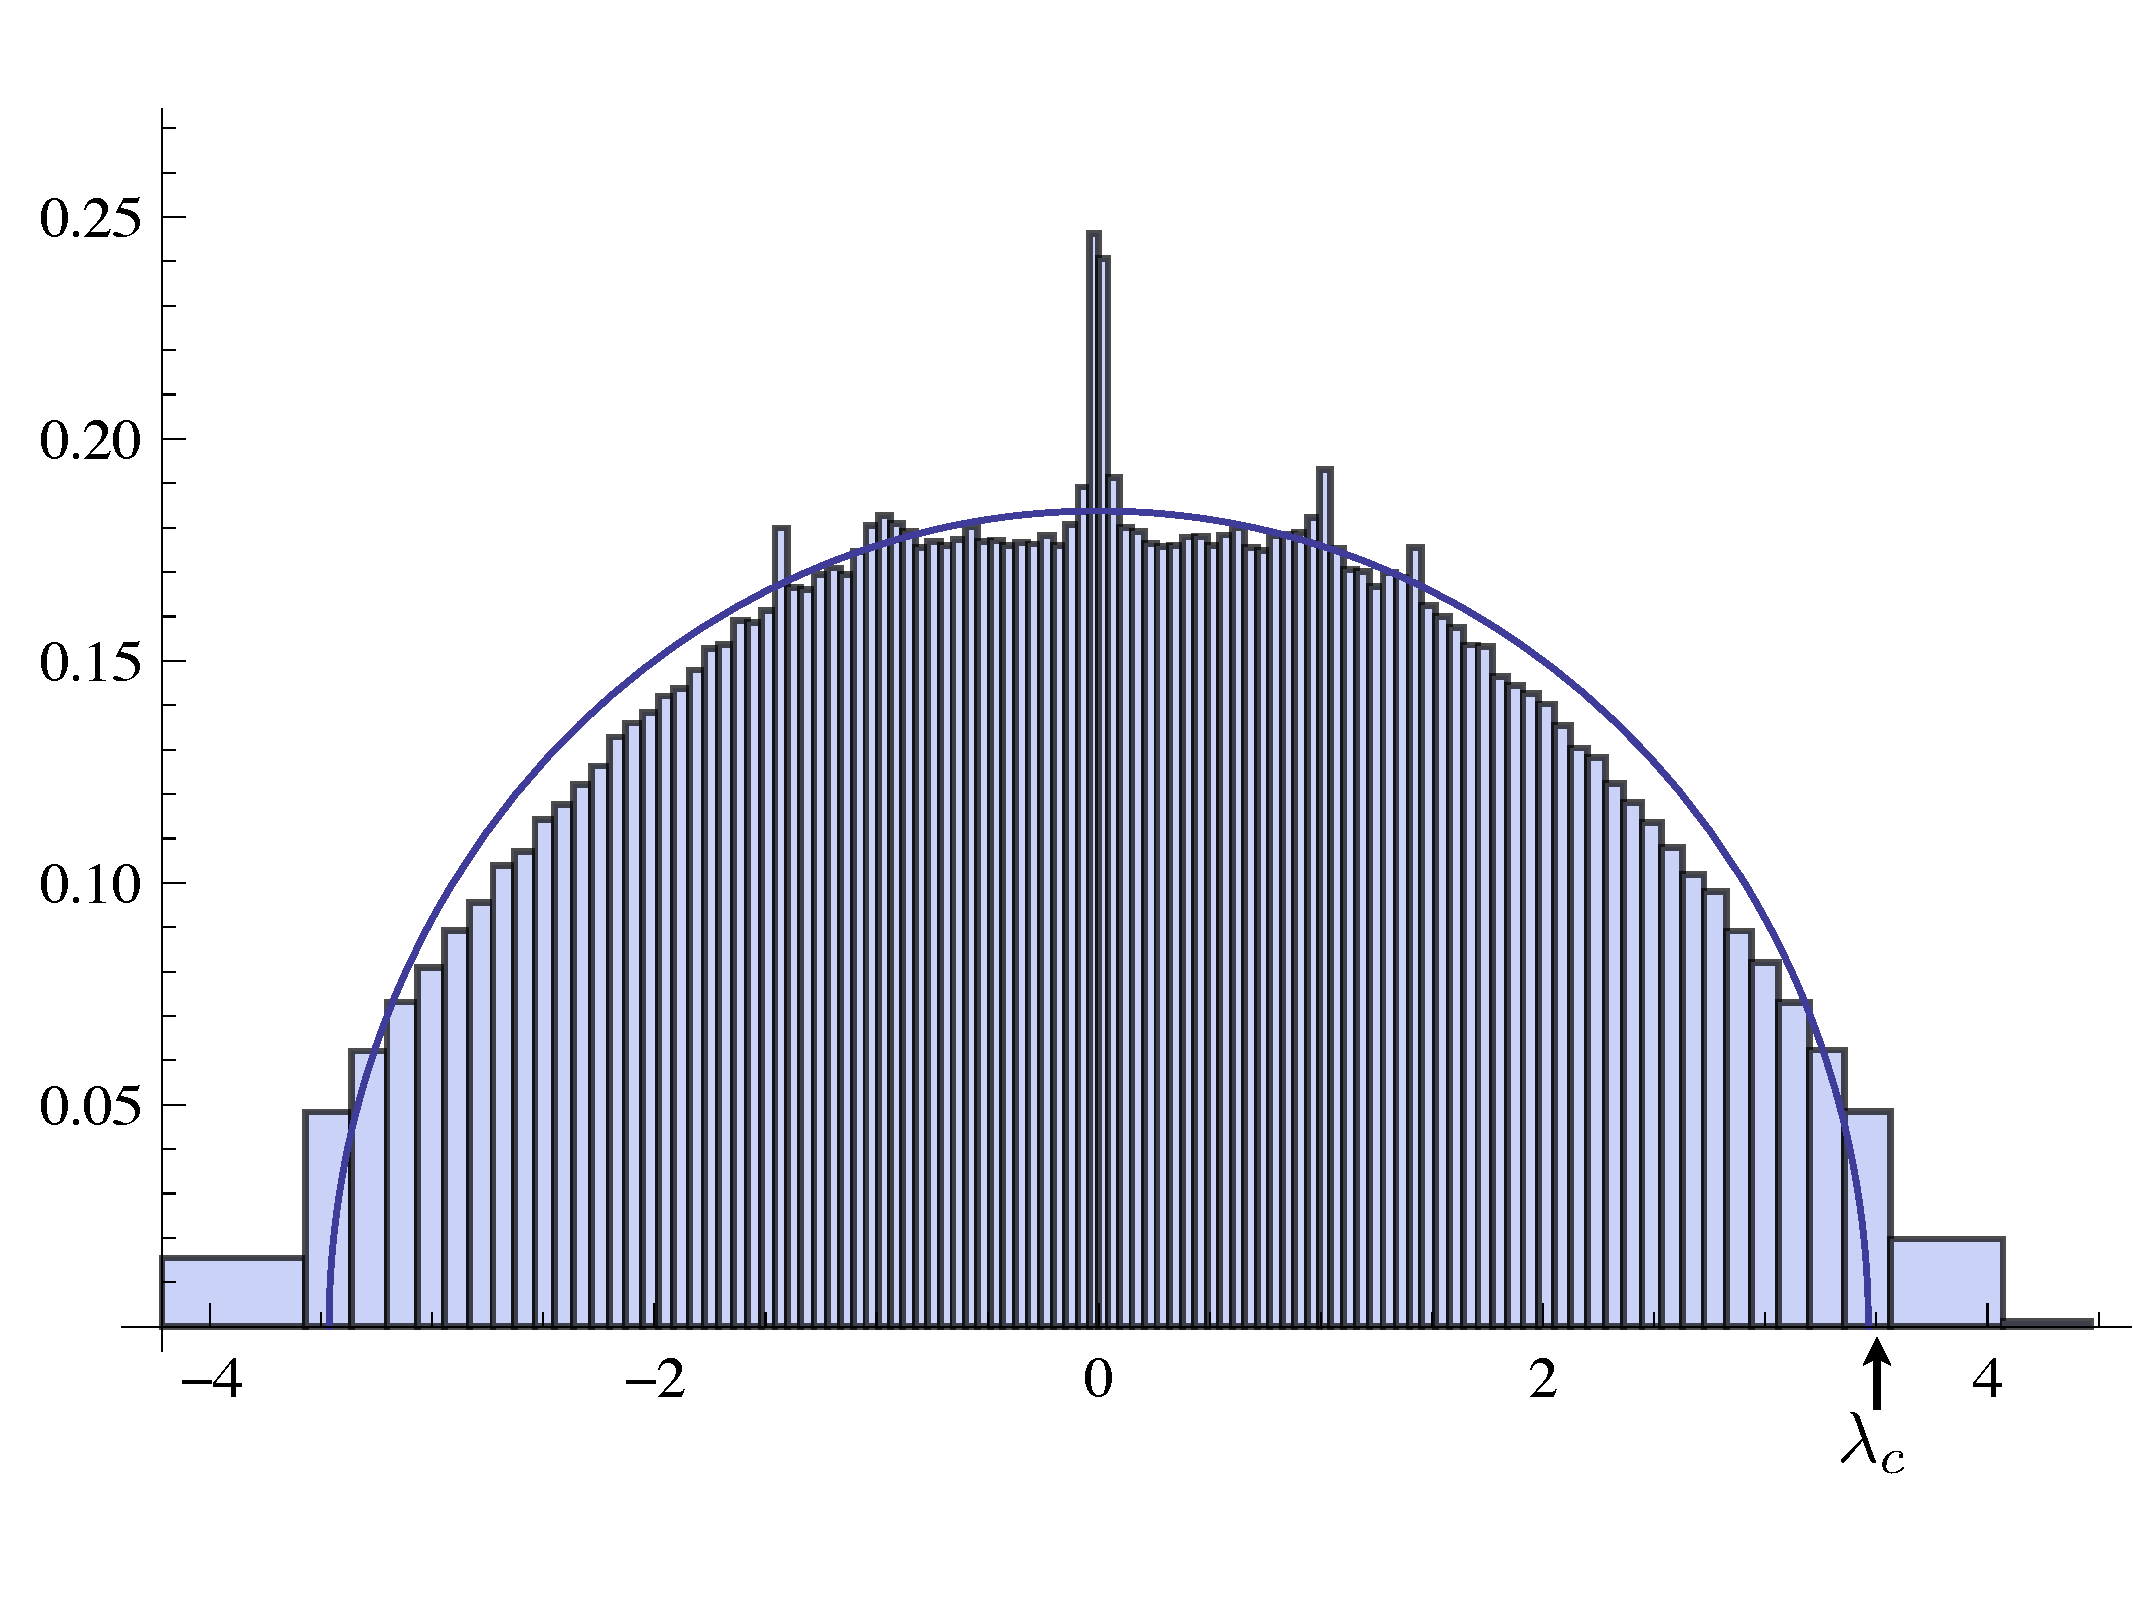
\includegraphics[width=1\textwidth]{EXP1}
			\label{exp1}
			\caption{The spectrum of $A$}
		\end{subfigure}
		\hspace{20pt}
		\begin{subfigure}[H]{0.45\textwidth}
			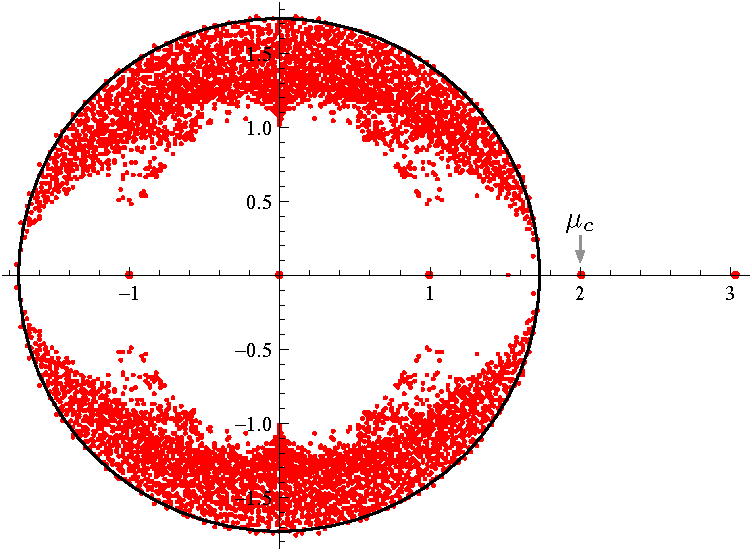
\includegraphics[width=1\textwidth]{EXP2}
			\label{exp2}
			\caption{The spectrum of $B$}
		\end{subfigure}
		}
		%\caption{The spectrum of $A$ (left) and $B$ (right)}
	\end{figure}
	\begin{itemize}
		\item $n = 4000$, $\cin = 5$, $\cout = 1$, $c = (\cin + \cout)/2 = 3$
		\item The radius of the bulk
			\begin{itemize}
				\item For $A$, $2\sqrt{c} = 3.46$
				\item For $B$, $\sqrt{c} = 1.73$
			\end{itemize}
	\end{itemize}
}
\note{
	\begin{itemize}
		\item SBM\ 的\ 参数
		\item 半圆\ 和\ 圆的半径
			\begin{itemize}
				\item 意义
				\item 取值
			\end{itemize}
		\item 第二大特征值\ $\lambda_c$\ 和\ $\mu_c$
	\end{itemize}
}

\frame{
	\frametitle{Experiments $n = 10^5$}	
	\begin{figure}
		\makebox[\linewidth][c]{
		\begin{subfigure}[H]{0.45\textwidth}
			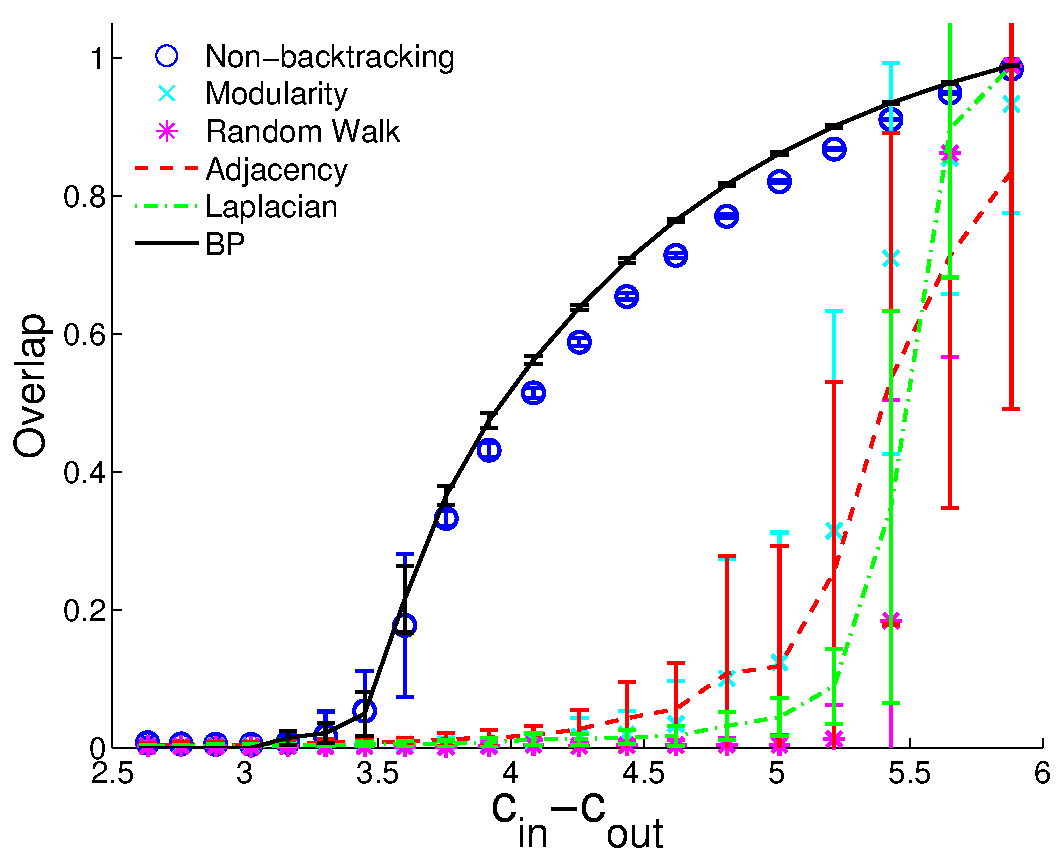
\includegraphics[width=1\textwidth]{EXP3}
			%\caption{The first 3 eigenvalues of $B$}
		\end{subfigure}
		\quad
		\begin{subfigure}[H]{0.45\textwidth}
			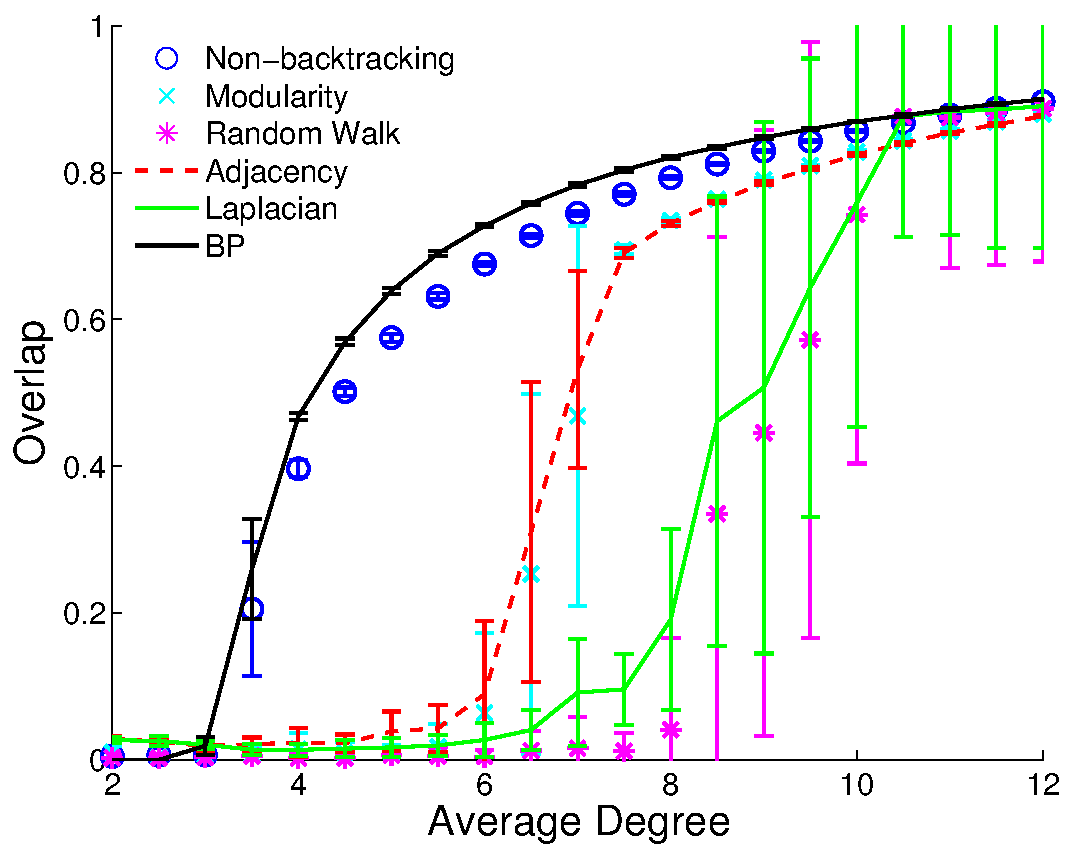
\includegraphics[width=1\textwidth]{EXP4}
		\end{subfigure}
		}
		%\caption{The accuracy of spectral clustering based on different matrices}
	\end{figure}
	\vspace{-5pt}
	\begin{itemize}
		%\item $n = 10^5$
			%\begin{itemize}
			%	\item On the left, set $c = 3$ and vary $\cin - \cout$
			%	\item On the right, set $\cout/\cin = 0.3$ and vary $c$
			%\end{itemize}
		\item $\mbox{Overlap} \triangleq
        \left( \frac{1}{n} \sum_u \delta_{g_u , \tilde{g}_u} -
          \frac{1}{q}\right) \Big{/} \left( 1 -  \frac{1}{q} \right)
$
		\vspace{5pt}
		\item Theoretical threshold\footnote[frame]{Elchanan Mossel, Joe Neeman, and Allan Sly (2012). Stochastic block models and
reconstruction. arXiv preprint, arXiv:1202.1499.} $\approx 3.46$
	\end{itemize}
}
\note{
	\begin{itemize}
		%\item 在\ SBM\ 生成的网络上\ 跑\ 不同的谱聚类方法
		\item 衡量标准:Overlap
		\item SBM\ 的\ 参数
			\begin{itemize}
				\item 左:$c = 3$,\ 增加\ $\cin - \cout$
				\item 右:$\cout / \cin = 0.3$, 增加\ $c$\
			\end{itemize}
		\item 理论阈值
	\end{itemize}
}

\frame{
	\frametitle{Detecting Number of Clusters}
	\begin{figure}
		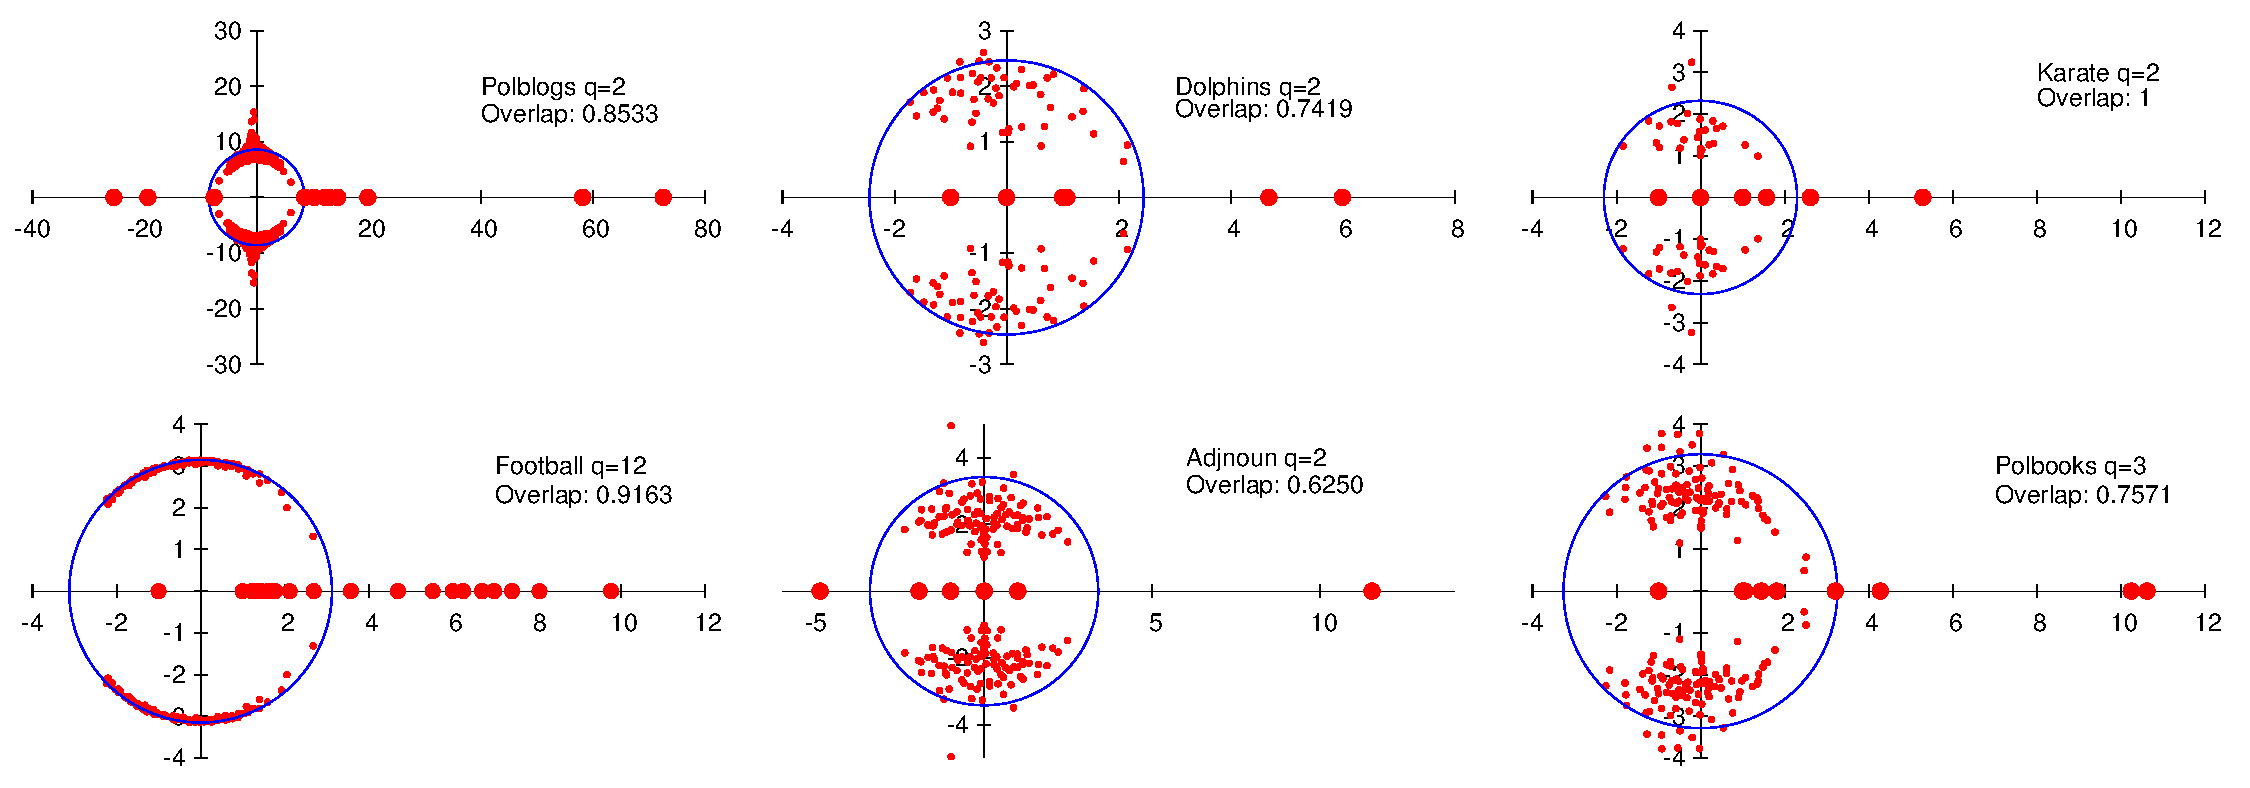
\includegraphics[width=1\textwidth]{DNOC}
		%\hspace*{8cm}
		\begin{itemize}
			\item Each circle's radius is $\sqrt{\rho(B)}$
			\item The number of real eigenvalues outside the circle indicates the number $q$ of clusters
		\end{itemize}
	\end{figure}
}
\note{
	\begin{itemize}
		\item 实际网络
		\item 检测社团个数
		\item 这一点\ Laplacian 或 Adjacency\ 都做不到
	\end{itemize}
}


\frame{
	\frametitle{Reducing the Computational Complexity}
	\vspace{-11.8pt}
	\begin{itemize}
		\item All eigenvalues $\lambda$ of $B$ not $\pm 1$ are the roots of the equation\footnote[frame]{Omer Angel, Joel Friedman, and Shlomo Hoory (2015). The non-backtracking spectrum of the universal cover of a graph. Trans. Amer. Math. Soc., 367(6):4287-4318.}
		\vspace{-10pt}
		\begin{equation} 
			\label{eq:ihara}
			\det[H(\lambda)] = \det \left[ \lambda^2 \id - \lambda A + (D-\id) \right] = 0 \,
		\end{equation}
		\item \vspace{-10pt} By the first companion linearization\footnote[frame]{Francoise Tisseur and Karl Meerbergen (2001). The quadratic eigenvalue problem. SIAM
Review, 43(2):235-286.}, roots of eq.~(\ref{eq:ihara}) are eigenvalues of \vspace{-10pt}
		\begin{equation}
			\label{eq:2nby2n}
			B' = \begin{pmatrix}
			0 & D-\id \\
			-\id & A
			\end{pmatrix}\quad \quad \quad \quad \nonumber
		\end{equation}
		\item \vspace{-2.5pt} Clustering by a $2n\times 2n$ matrix rather than a $2m\times 2m$ one
	\end{itemize}
}

\frame{
	\frametitle{The Bethe Hessian Matrix}
	\vspace{-9pt}
	\begin{itemize}
		\item All eigenvalues $\lambda$ of $B$ not $\pm 1$ are the roots of the equation
		\vspace{-10pt}
		\begin{equation} 
			\label{eq:ihara}
			\det[H(\lambda)] =  \det \left[ \lambda^2 \id - \lambda A + (D-\id) \right] = 0 \,
			\tag{1}
		\end{equation}
	\item The Bethe Hessian matrix $H(r)$
			\[
				\quad \ \ H(r):=r^2\id-rA+(D - \id) %\quad \quad  \quad \quad \quad
			\]
			\item $\forall$ real eigenvalue $\lambda$ of $B$, $H(\lambda)$ has a eigenvalue 0
			\begin{itemize}
				\item $H(\lambda\only<1-1>{\hspace{4.75pt}}\only<2-2>{_2})$'s null space \hspace{2pt} $\longleftrightarrow$ \hspace{2pt} $B$'s eigenvector corresponding to $\lambda\only<1-1>{\hspace{4.75pt}}\only<2-2>{_2}$
				\item Let $r_c = \sqrt{\rho(B)}$
				\item Eigenvectors of $H(r_c)$'s negative eigenvalues reveal clustering
			\end{itemize}
	\end{itemize}
}

\frame{
	\frametitle{Spectrum of $B$ and $H(r)$}
	\vspace{-20pt}
	\begin{wrapfigure}{L}{0.55\textwidth}
		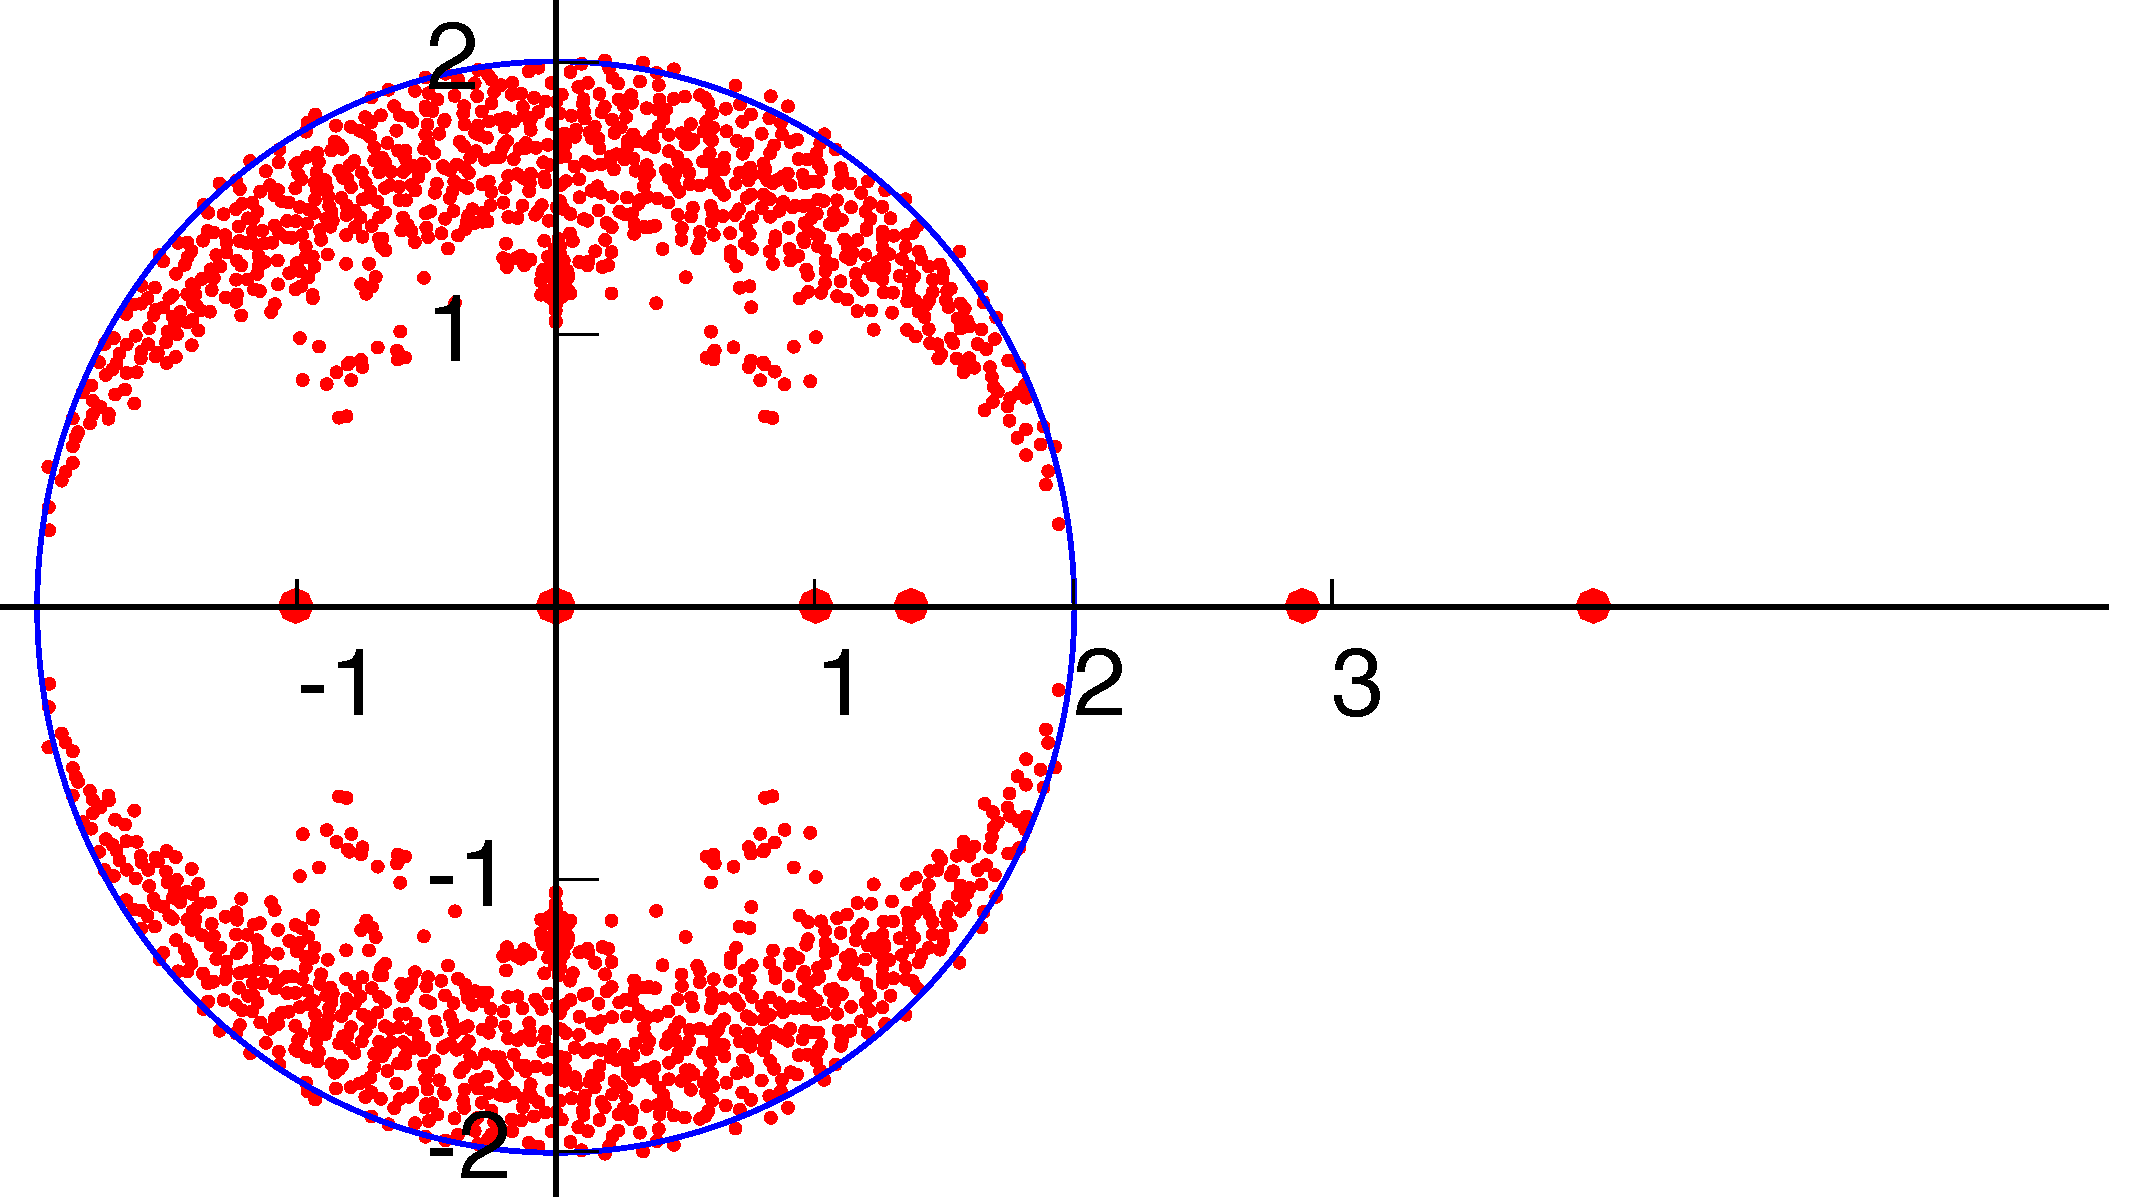
\includegraphics[width=0.5\textwidth]{1000}
	\end{wrapfigure}
	\quad \\[2.5pt]
	Stochastic block model
	\begin{itemize}
		\item $n = 10^4$
		\item $c = 4$
		\item $\cout / \cin = \frac{1}{7}$
	\end{itemize}
	\quad \\[5pt]
	\insfig{AE}
}

\frame{
	\frametitle{Experiments}
	\insfig{EXB1}
	\insfig[0.8]{EXB2}
}

\frame{
	\frametitle{Conclusions} % and Perspectives}
	\begin{itemize}
		\item Comparing to non-backtracking clustering
			\begin{itemize}
				\item $H(r_c)$ is $n\times n$ symmetric, while $B'$ is $2n\times 2n$ non-symmetric
				\item Need to compute $\rho(B)$ to calculate $r_c = \sqrt{\rho(B)}$
					\begin{itemize}
						\item By solving quadratic eigenproblem~(\ref{eq2}) using a SLP algorithm\footnote[frame]{Axel Ruhe (1973). Algorithms for the nonlinear eigenvalue problem. SIAM Journal on
Numerical Analysis, 10(4):674–689.} \vspace{-5pt}
\begin{equation}
	\label{eq2}
	\det{H(\lambda)} = \det{\left[\lambda^2\id-\lambda A+(D-\id)	\right]} = 0 \quad \quad %\quad %\quad
\end{equation}
			\end{itemize}
		\end{itemize}
		\item \vspace{-5pt} Detecting the communities in sparse network
			\begin{itemize}
				\item All the way down to the threshold in SBM
			\end{itemize}
		\item The number of negative eigenvalues indicating the number of clusters
	\end{itemize}
}

\begin{frame}
	\Huge{\centerline{The End}}
\end{frame}

%\begin{thebibliography}{9}
%\bibitem{ClFi07}
%J.~Clark and R.~Fierro, ``Mobile robotic sensors for perimeter detection and
%  tracking,'' \emph{ISA Trans.}, vol.~46, no.~1, pp. 3--13, 2007.
%\end{thebibliography}

\end{spacing}
\end{document}